\documentclass[twocolumn]{article}

\usepackage{graphicx}
\usepackage[hidelinks]{hyperref}
\usepackage[english]{babel}
\usepackage{amsmath}
\usepackage[table]{xcolor}
\usepackage{tikz}
\usepackage{pgfplots}
\usepackage{xifthen}
\usepackage{caption}
\captionsetup{font=footnotesize}
\usepackage{xspace}
\usepackage{enumitem}
\usepackage[textwidth=1.7cm,textsize=small]{todonotes}
\usepackage{import}
\usepackage{natbib}
\usepgfplotslibrary{colorbrewer}
\usepackage{authblk}
\usepackage{booktabs}
\usepackage{bm}
\usepackage{subcaption}
\usepackage{datatool}
\usepackage{cleveref}
\usepackage{soul}
\usepackage{siunitx}

% General Math Notation
\def\vct#1{\bm{#1}}  % vectors in bold
\def\trans{\intercal}  % matrix transpose symbol

% Our Method
\def\ours{\textsc{Blinx}\xspace}
\def\lbfcs{\textsc{lbFCS+}\xspace}
\def\qpaint{\textsc{qPAINT}\xspace}

% Variables
\def\n{\ensuremath{n}\xspace}                 % count
\def\ndist{\ensuremath{\vct{n}}\xspace}       % distribution of predictions
\def\truen{\ensuremath{n^*}\xspace}           % true count
\def\estimatedn{\ensuremath{\hat{n}}\xspace}  % estimated count
\def\z#1{\ensuremath{z_{#1}}\xspace}          % number of active emitters at time t: \y{t}
\def\x#1{\ensuremath{x_{#1}}\xspace}          % intensity at time t: \x{t}
\def\xp#1{\ensuremath{\tilde{x}_{#1}}\xspace} % intensity at time t in photon space: \xp{t}
\def\states{\ensuremath{\vct{z}}\xspace}      % all active emitters over time
\def\trace{\ensuremath{\vct{x}}\xspace}       % all intensities over time
\def\pon{\ensuremath{p_\text{on}}\xspace}     % prob. for activating
\def\poff{\ensuremath{p_\text{off}}\xspace}   % prob. for deactivating
\def\re{\ensuremath{r_e}\xspace}              % fluorophore emission rate
\def\rb{\ensuremath{r_b}\xspace}              % background emission rate
\def\camoffset{\ensuremath{\mu}\xspace}       % camera offset
\def\camvar{\ensuremath{\sigma^2}\xspace}       % camera variance
\def\camgain{\ensuremath{g}\xspace}           % camera gain
\def\parameters{\ensuremath{\theta}\xspace}   % all parameters (mu, sigma, ...)
\def\parameterst{\ensuremath{\parameters_T}}  % transition parameters
\def\parameterse{\ensuremath{\parameters_E}}  % emission parameters
\def\parametersc{\ensuremath{\parameters_C}}  % camera parameters
\def\photons{\ensuremath{c}\xspace}           % number of photons per spot
\def\deltat{\ensuremath{\Delta t}\xspace}     % length of frame

\def\pchain{\ensuremath{\alpha\xspace}}       % recursive probability for forward algorithm
\def\pchainnorm{\ensuremath{\tilde{\alpha}\xspace}}
                                              % \pchain normalized
\def\norms{\ensuremath{\beta\xspace}} % normalization factors for \pchain
\def\object{object} % what to call things we want to count
\def\objects{objects} % what to call things we want to count plural
\def\smallobjects{subunits} % what to call things we want to count plural

\DeclareMathOperator{\poisson}{Poisson}

% Functions
%\newcommand{\argmax}[1]{\mathop{\arg\max}_{#1}\hspace{0.5em}}

\usetikzlibrary{arrows}
\usetikzlibrary{arrows.meta}
\usetikzlibrary{backgrounds}
\usetikzlibrary{calc}
\usetikzlibrary{chains}
\usetikzlibrary{decorations.markings}
\usetikzlibrary{decorations.pathmorphing}
\usetikzlibrary{fit}
\usetikzlibrary{matrix}
\usetikzlibrary{mindmap}
\usetikzlibrary{pgfplots.colormaps}
\usetikzlibrary{positioning}
\usetikzlibrary{shadows}
\usetikzlibrary{shapes}
\usetikzlibrary{trees}

\newlength\patchwidth
\newlength\intrasamplerowsep
\newlength\intersamplerowsep

% monochrome
\definecolor{funkey_bright}{HTML}{FFFFFF}
\definecolor{funkey_lightgrey}{HTML}{cccccc}
\definecolor{funkey_grey}{HTML}{666666}

% principal colors
\definecolor{funkey_color_1}{HTML}{834D9D}  % purple
\definecolor{funkey_color_2}{HTML}{F2A431}  % orange
\definecolor{funkey_color_3}{HTML}{55B849}  % green
\definecolor{funkey_color_4}{HTML}{DB8457}  % peach
\definecolor{funkey_color_5}{HTML}{8174B1}  % lavender
\definecolor{funkey_color_6}{HTML}{ADD8E6}  % aquamarine
\definecolor{funkey_color_7}{HTML}{000080}  % dark blue
\definecolor{funkey_color_8}{HTML}{800020}  % dark red
\definecolor{funkey_color_9}{HTML}{228B22}  % dark green
\definecolor{funkey_color_10}{HTML}{F5C108} % lemon
\definecolor{funkey_color_11}{HTML}{DA3074} % dirty pink
\definecolor{funkey_color_12}{HTML}{CC00FF} % electric purple
\definecolor{funkey_color_13}{HTML}{FF9900} % deep orange
\definecolor{funkey_color_14}{HTML}{006666} % teal blue
\definecolor{funkey_color_15}{HTML}{660066} % dark magenta

% background color
\colorlet{funkey_dark}{purple!10!black}

% how to use colors in funkey theme
\colorlet{funkey_highlight}{funkey_color_2}
\colorlet{funkey_textcolor}{funkey_bright}
\colorlet{funkey_bg}{funkey_dark}
\colorlet{funkey_alt_bg}{funkey_lightgrey}


\tikzstyle{real}=[rectangle,rounded corners,line width=1pt,draw=funkey_grey]
\tikzstyle{stylesource}=[rectangle,rounded corners,line width=1pt,dashed,draw=funkey_grey]
\tikzstyle{counterfactual}=[rectangle,rounded corners,line width=1pt,draw=funkey_color_1,fill=funkey_color_1!10!white]

%%%%%%%%%%%
% GENERAL %
%%%%%%%%%%%
\tikzstyle{icon}=[rectangle,rounded corners,draw=funkey_lightgrey,thick]

\tikzstyle{var}=[circle,draw=funkey_lightgrey,minimum width=7mm]
\tikzstyle{fun}=[rectangle,draw=funkey_lightgrey,minimum width=7mm]
\tikzstyle{loss}=[rectangle,rounded corners,thick,fill opacity=0.2]

\tikzstyle{neuron}=[circle,fill=funkey_color_2,inner sep=0.7mm]
\tikzstyle{synapse}=[->,>=latex',funkey_color_1,thick]

\tikzstyle{inset}=
  [rectangle,inner sep=0,clip]
\tikzstyle{image}=
  [inner sep=0,outer sep=0,draw=funkey_lightgrey]
\tikzstyle{candidate}=
  [very thick,funkey_color_1,->,shorten >=2mm]
\tikzstyle{cell}=
  [circle,inner sep=3pt,fill]

\tikzstyle{data}=
  [rectangle,rounded corners,draw,fill=funkey_lightgrey]
\tikzstyle{method}=
  [rectangle,rounded corners,fill=funkey_color_1,text=funkey_bright,text width=5mm,align=center]
\tikzstyle{arrow}=
  [-{Latex[round]}]

\tikzstyle{process}=
  [single arrow,fill=funkey_lightgrey,inner sep=2pt,minimum height=5mm,single arrow head extend=1.5mm]

\tikzstyle{perceptron}=
  [circle,outer color=orange!50!white,inner color=white]
\tikzstyle{perceptron_input}=
  [circle,outer color=blue!20!white, inner color=white,anchor=base]
\tikzstyle{perceptron_output}=
  [circle,outer color=blue!20!white, inner color=white,anchor=base]
\tikzstyle{operator}=
  [circle,draw=lightgray,fill=white,inner sep=1pt]
\tikzstyle{connection}=
  [draw=lightgray,thin]
\tikzstyle{annotation}=
  [rectangle,rounded corners,draw=lightgray,fill=white,fill opacity=0.7,text opacity=1]

\tikzstyle{fmap}=
  [perceptron_input,rectangle,draw=blue!25!white]

\tikzstyle{box}=
  [rectangle,rounded corners,minimum width=3mm]

\tikzstyle{kernel}=
  [draw=gray,fill=blue!10!white]
\tikzstyle{bb}=
  [inner sep=0,outer sep=0]

\tikzstyle{unet_l1}=[]
\tikzstyle{unet_l2}=
  [scale=0.7,transform shape]
\tikzstyle{unet_l3}=
  [scale=0.5,transform shape]
\tikzstyle{unet_l4}=
  [scale=0.5,transform shape]

\tikzstyle{unet_annotation}=
  [circle,fill=white,draw=black,text=black,minimum width=4mm]

\tikzstyle{conv_pass}=
  [single arrow,shading=axis,left color=blue!50!white, right color=blue!10!white,draw=blue!50!white!70!black, inner sep=0]

\tikzstyle{copy_pass}=
  [single arrow,shading=axis,left color=purple!50!white, right color=purple!10!white,draw=purple!50!white!70!black, inner sep=0]

\tikzstyle{max_pool_pass}=
  [single arrow,shading=axis,left color=orange!50!white, right color=orange!10!white,draw=orange!50!white!70!black, inner sep=0]

\tikzstyle{upsampling_pass}=
  [single arrow,shading=axis,left color=brown!50!white, right color=brown!10!white,draw=brown!50!white!70!black, inner sep=0]

\tikzstyle{frame}=
  [rectangle,draw,fill=black]

%\tikzstyle{hand}=[decorate,decoration={random steps,segment length=2pt,amplitude=0.2pt}]
%\tikzstyle{perceptron}=
  %[circle,outer color=orange!50!white,inner color=white,hand]
%\tikzstyle{perceptron_input}=
  %[circle,draw=black,hand,fill=white]
%\tikzstyle{perceptron_output}=
  %[circle,draw=black,hand,fill=white]
%\tikzstyle{operator}=
  %[circle,draw=black,hand,fill=white]

\tikzstyle{pointer}=
  [->,thick,funkey_highlight]

\tikzstyle{gp_node}=
  [circle,draw,fill=gray!10!white,minimum width=0.5cm]
\tikzstyle{gp_annotation}=
  [rectangle,rounded corners,draw=gray!20!white,fill=gray!10!white,minimum width=0.5cm]

\tikzstyle{gp_edge}=
  [->,>=stealth',thick]
\tikzstyle{gp_request_edge}=
  [->,>=stealth',color=blue!50!white]
\tikzstyle{gp_batch_edge}=
  [->,>=stealth',color=orange!50!white]

\tikzstyle{gp_request}=
  [rectangle,rounded corners,fill=white,draw=gray]

%%%%%%%%%%
% MACROS %
%%%%%%%%%%

\newcommand{\getzoomfactor}{%
\pgfgettransformentries{\myxscale}{\@tempa}{\@tempa}{\myyscale}{\@tempa}{\@tempa}
\gdef\zoomfactor{\myxscale}
}

\def\scalebar#1#2{%
  \fill[black] (0,0) rectangle ($(#1,-#1*0.2)$);
  \path (0,0) -- node[above] {#2} (#1,0);
}

\pgfplotsset{compat=1.15}
\usetikzlibrary{pgfplots.groupplots}
\usepgfplotslibrary{statistics}
\usepgfplotslibrary{patchplots}

\pgfplotsset{
  errors/.style={
    stack plots=y,
    area style,
    enlarge x limits=false,
    xmajorgrids=true,
    ymajorgrids=true,
    yminorgrids=true,
    legend reversed
  }
}

\pgfplotsset{
  discard if not/.style args={#1 is #2}{
    x filter/.code={
      \edef\tempa{\thisrow{#1}}
      \edef\tempb{#2}
      \ifx\tempa\tempb
      \else
        \def\pgfmathresult{inf}
      \fi
    }
  }
}

\pgfplotsset{
  discard if not both/.style args={#1 is #2 and #3 is #4}{
    x filter/.code={
      \edef\tempa{\thisrow{#1}}
      \edef\tempb{#2}
      \edef\tempc{\thisrow{#3}}
      \edef\tempd{#4}
      \ifx\tempa\tempb
        \ifx\tempc\tempd
        \else
          \def\pgfmathresult{inf}
        \fi
      \else
        \def\pgfmathresult{inf}
      \fi
    }
  }
}

\pgfplotsset{
  discard if not all three/.style args={#1 is #2 and #3 is #4 and #5 is #6}{
    x filter/.code={
      \edef\tempa{\thisrow{#1}}
      \edef\tempb{#2}
      \edef\tempc{\thisrow{#3}}
      \edef\tempd{#4}
      \edef\tempe{\thisrow{#5}}
      \edef\tempf{#6}
      \ifx\tempa\tempb
        \ifx\tempc\tempd
          \ifx\tempe\tempf
          \else
            \def\pgfmathresult{inf}
          \fi
        \else
          \def\pgfmathresult{inf}
        \fi
      \else
        \def\pgfmathresult{inf}
      \fi
    }
  }
}
\pgfmathdeclarefunction{invgauss}{2}{%
  \pgfmathparse{sqrt(-2*ln(#1))*cos(deg(2*pi*#2))}%
}

\def\tikzmath#1#2{\tikz[remember picture,baseline=(#1.base),inner sep=0pt] \node (#1) {$\displaystyle #2$};}

\newenvironment{panel}[2]{%
  \begin{minipage}[t][][t]{#2}%
    \strut#1%

    \vspace{-\baselineskip}%
}{%
  \end{minipage}%
}%
\newenvironment{panelcolumn}[1]{%
  \begin{minipage}[t][][t]{#1}%
}{%
  \end{minipage}%
}%

% useful for setting/computing the width of plots
\newlength{\plotwidth}
\newlength{\plotheight}

% draw 5 example fluorophores, args are "on" or "off"
\def\blinky#1#2#3#4#5{
  \begin{tikzpicture}[node distance=3mm]
    \node[site#1] (s1) {};
    \node[site#2,right of=s1] (s2) {};
    \coordinate (s12) at ($(s1)!.5!(s2)$);
    \node[site#3,right of=s2] (s3) {};
    \node[site#4,below of=s12] (s4) {};
    \node[site#5,right of=s4] (s5) {};
    \foreach \angle in {0, 45, 90, 135, 180, 225, 270, 315}{
      \begin{scope}[rotate=\angle]
        \draw[sitelight#1] ($(s1)+(0,0.13)$) -- ($(s1)+(0,0.16)$);
        \draw[sitelight#2] ($(s2)+(0,0.13)$) -- ($(s2)+(0,0.16)$);
        \draw[sitelight#3] ($(s3)+(0,0.13)$) -- ($(s3)+(0,0.16)$);
        \draw[sitelight#4] ($(s4)+(0,0.13)$) -- ($(s4)+(0,0.16)$);
        \draw[sitelight#5] ($(s5)+(0,0.13)$) -- ($(s5)+(0,0.16)$);
      \end{scope}
    }
  \end{tikzpicture}
}

% continued caption texts
%
% Usage:
%\begin{figure}
%  \input{figure sources}
%  \caption{
%    ...
%    \captbc
%  }
%\end{figure}
%\begin{figure}
%  \contcaption{
%    \capcont
%    ...
%  }
%  \label{goes here}
%\end{figure}
\def\captbc{\emph{(caption continued on next page)}\xspace}
\def\capcont{\emph{(continued)\ }}


% references
\def\figref#1{Fig.~\ref{#1}}
\def\subfigref#1{(\subref{#1})}
\def\secref#1{Section~\ref{#1}}
\def\tabref#1{Table~\ref{#1}}
\def\eqref#1{(\ref{#1})}

% common abbreviations
\newcommand{\eg}{\emph{e.g.}\xspace}
\newcommand{\ie}{\emph{i.e.}\xspace}

% todo notes with \todo{}
\let\todonote\todo%
\renewcommand{\todo}[1]{\todonote[color=orange!50!white]{\footnotesize #1}\xspace}

% introduce a new word
%\def\introduce#1{{\color{funkey_color_1}\ul{#1}}}
\def\introduce#1{#1}  % uncomment this for final version

% prefer JPG when available
\usepackage{grfext}
\PrependGraphicsExtensions*{.jpg,.JPG}

% evaluate a mathematical expression #2 and assign the result to macro #1
\def\mathlet#1#2{\pgfmathparse{#2}\let#1\pgfmathresult}

% set text in tikz node
\newcommand{\tikztext}[2]{\tikz[baseline]\node[anchor=base,inner sep=0] (#1) {#2};}

% General Math Notation
\def\vct#1{\bm{#1}}  % vectors in bold
\def\trans{\intercal}  % matrix transpose symbol

% Our Method
\def\ours{\textsc{Blinx}\xspace}
\def\lbfcs{\textsc{lbFCS+}\xspace}
\def\qpaint{\textsc{qPAINT}\xspace}

% Variables
\def\n{\ensuremath{n}\xspace}                 % count
\def\ndist{\ensuremath{\vct{n}}\xspace}       % distribution of predictions
\def\truen{\ensuremath{n^*}\xspace}           % true count
\def\estimatedn{\ensuremath{\hat{n}}\xspace}  % estimated count
\def\z#1{\ensuremath{z_{#1}}\xspace}          % number of active emitters at time t: \y{t}
\def\x#1{\ensuremath{x_{#1}}\xspace}          % intensity at time t: \x{t}
\def\xp#1{\ensuremath{\tilde{x}_{#1}}\xspace} % intensity at time t in photon space: \xp{t}
\def\states{\ensuremath{\vct{z}}\xspace}      % all active emitters over time
\def\trace{\ensuremath{\vct{x}}\xspace}       % all intensities over time
\def\pon{\ensuremath{p_\text{on}}\xspace}     % prob. for activating
\def\poff{\ensuremath{p_\text{off}}\xspace}   % prob. for deactivating
\def\re{\ensuremath{r_e}\xspace}              % fluorophore emission rate
\def\rb{\ensuremath{r_b}\xspace}              % background emission rate
\def\camoffset{\ensuremath{\mu}\xspace}       % camera offset
\def\camvar{\ensuremath{\sigma^2}\xspace}       % camera variance
\def\camgain{\ensuremath{g}\xspace}           % camera gain
\def\parameters{\ensuremath{\theta}\xspace}   % all parameters (mu, sigma, ...)
\def\parameterst{\ensuremath{\parameters_T}}  % transition parameters
\def\parameterse{\ensuremath{\parameters_E}}  % emission parameters
\def\parametersc{\ensuremath{\parameters_C}}  % camera parameters
\def\photons{\ensuremath{c}\xspace}           % number of photons per spot
\def\deltat{\ensuremath{\Delta t}\xspace}     % length of frame

\def\pchain{\ensuremath{\alpha\xspace}}       % recursive probability for forward algorithm
\def\pchainnorm{\ensuremath{\tilde{\alpha}\xspace}}
                                              % \pchain normalized
\def\norms{\ensuremath{\beta\xspace}} % normalization factors for \pchain
\def\object{object} % what to call things we want to count
\def\objects{objects} % what to call things we want to count plural
\def\smallobjects{subunits} % what to call things we want to count plural

\DeclareMathOperator{\poisson}{Poisson}

% Functions
%\newcommand{\argmax}[1]{\mathop{\arg\max}_{#1}\hspace{0.5em}}


\begin{document}

\title{A Bayesian Solution to the Molecular Counting Problem}

\author{
  Alexander Hillsley$^{1}$,
  Johannes Stein$^{2}$,
  Paul Tillberg$^{1}$,
  David Stern$^{1}$,
  Jan Funke$^{1}$\thanks{Corresponding Author}
  \\\\
  \normalsize{$^1$ HHMI Janelia Research Campus, Ashburn, VA},
  \normalsize{$^2$ Wyss Institute, Harvard University, Boston, MA}
}

\maketitle

\begin{figure*}

  \begin{panel}{(a)}{\textwidth}
    \vspace{5mm}
    \small
    \tikzsetnextfilename{figure_1_overview}
    \usetikzlibrary{spy}%
\def\blinky#1#2#3#4#5{%
  \begin{tikzpicture}[node distance=3mm]
    \node[site#1] (s1) {};
    \node[site#2,right of=s1] (s2) {};
    \coordinate (s12) at ($(s1)!.5!(s2)$);
    \node[site#3,right of=s2] (s3) {};
    \node[site#4,below of=s12] (s4) {};
    \node[site#5,right of=s4] (s5) {};
    \foreach \angle in {0, 45, 90, 135, 180, 225, 270, 315}{
      \begin{scope}[rotate=\angle]
        \draw[sitelight#1] ($(s1)+(0,0.13)$) -- ($(s1)+(0,0.16)$);
        \draw[sitelight#2] ($(s2)+(0,0.13)$) -- ($(s2)+(0,0.16)$);
        \draw[sitelight#3] ($(s3)+(0,0.13)$) -- ($(s3)+(0,0.16)$);
        \draw[sitelight#4] ($(s4)+(0,0.13)$) -- ($(s4)+(0,0.16)$);
        \draw[sitelight#5] ($(s5)+(0,0.13)$) -- ($(s5)+(0,0.16)$);
      \end{scope}
    }
  \end{tikzpicture}
}%
\begin{tikzpicture}

  \begin{scope}[spy using outlines={magnification=2,size=12mm,very thick}]

    \node[image] (frame) {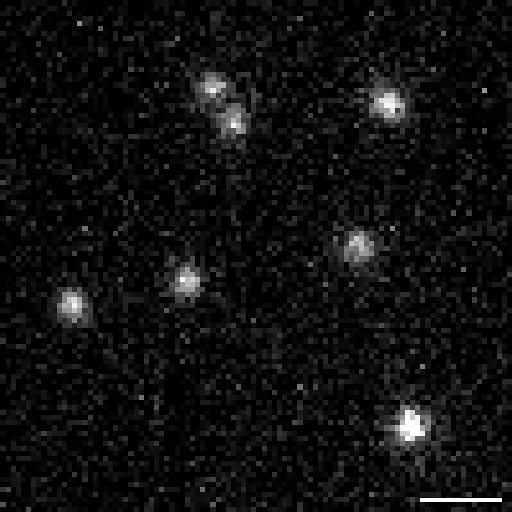
\includegraphics[width=4cm]{figures/data/overview/sample_frame}};

    \spy on ($(frame)+(1.1, 1.2)$)
      in node (patch_3) [image,right=6mm,anchor=north west]
      at (frame.north east);
    \spy on ($(frame)+(0.9, 1.1)$)
      in node (patch_2) [image,right=6mm,anchor=north west]
      at ($(frame.north east)-(0.1,0.1)$);
    \spy[
        draw=funkey_color_1,
        every spy on node/.append style={ultra thick},
        every spy in node/.append style={ultra thick},
        spy connection path={\draw[ultra thick] (tikzspyonnode) -- (tikzspyinnode);}
    ]
      on ($(frame)+(1.0, 1.2)$)
      in node (patch_1) [image,right=6mm,anchor=north west]
      at ($(frame.north east)-(0.2,0.2)$);
  \end{scope}

  % example trace
  \node[right=4mm,anchor=north west,text width=6cm,inner sep=0] (trace) at (patch_3.north east) {%
    \def\tracecsv{figures/data/overview/trace.csv}%
    \def\traceintensitycol{trace}%
    \def\nolabels{}%
    \tikzexternaldisable%
    \centerline{\begin{tikzpicture}%
  \begin{axis}[
    name=trace,
    width=0.8\textwidth,
    height=5cm,
    xlabel=frames,
    ylabel=intensity,
    enlarge x limits=false,
    xtick distance=500,
    grid=major,
    grid style={dashed},
    scaled ticks=false,
    ticklabel style={font=\small},
    legend style={nodes={scale=0.6, transform shape}},
  ]

    \addplot [
      color=tracecolor,
      mark=*,
      mark size=0.7pt,
      mark options={line width=0},
      fill opacity=0.8,
      draw opacity=0.2,
    ] table [
      col sep=comma,
      x=frames,
      y=\traceintensitycol
    ] {\tracecsv};
    \addlegendentry{intensity trace}

    \addplot [
      color=ztracecolor,
      thick
    ] table [
      col sep=comma,
      x=frames,
      y=\zcol
    ] {\tracecsv};
    \addlegendentry{inferred state}

    % remember min/max y-axis values for next plot
    \pgfplotsextra{
      \pgfmathparse{\pgfkeysvalueof{/pgfplots/ymin}}
      \global\let\ymin\pgfmathresult
      \pgfmathparse{\pgfkeysvalueof{/pgfplots/ymax}}
      \global\let\ymax\pgfmathresult
    }

  \end{axis}

  \begin{axis}[
    at={($(trace.east) + (4mm,0)$)},
    anchor=west,
    width=0.3\textwidth,
    height=5cm,
    yticklabel=\empty,
    xtick distance=0.005,
    xlabel=probability,
    grid=major,
    grid style={dashed, very thin},
    enlarge x limits={value=0.1,upper},
    scaled ticks=false,
    ymin=\ymin,
    ymax=\ymax,
    ticklabel style={font=\small},
    legend style={nodes={scale=0.6, transform shape}},
  ]

    \addplot+[
      xbar interval,
      mark=none,
      color=tracecolor,
      fill=tracecolor,
      fill opacity=0.6,
      draw=none,
    ] table [
      col sep=comma,
      y=\histbincol,
      x=\histcountcol,
    ] {\histogramcsv};
    \addlegendentry{intensity histogram}

    \addplot[
      color=intensitymodelcolor!80!black,
      thick
    ] table [
      col sep=comma,
      y=\histbincol,
      x=\modelfitcol
    ] {\histogramcsv};
    \addlegendentry{inferred model}

  \end{axis}
\end{tikzpicture}%
}%
    \tikzexternalenable%
  };
  \node[anchor=north,inner sep=0pt] at (trace.230) {\tiny time};
  \node[rotate=90,anchor=south,inner sep=1pt] at (trace.west) {\tiny intensity};

  % observed / hidden line
  \draw[gray,very thick]
    (patch_1.west|-frame.355) --
      node[pos=0,anchor=south west] {observed}
      node[pos=0,anchor=north west] {hidden}
      node[pos=0.35] (sample_1) {}
      node[pos=0.60] (sample_2) {}
      node[pos=0.96] (sample_3) {}
    (trace.east|-frame.355);

  % brace to MLE
  \draw[decorate,decoration={brace,raise=2mm}]
    (trace.north east) --
    node[pos=0.5,right=5mm,draw,rectangle,rounded corners] (mle) {\ours}
    (trace.south east);

  % posterior
  \node[anchor=north west,text width=3.6cm] (posterior) at ($(trace.north east)+(1.8,0.3)$) {%
    \def\posteriorcsv{figures/data/overview/posterior.csv}%
    \def\posteriorcol{posterior}%
    \def\noylabels{}%
    \tikzexternaldisable%
    \@ifundefined{noylabels}{}{%
  \pgfplotsset{yticklabel=\empty}%
}%
\begin{tikzpicture}%

  \def\eps{0.001}

  \begin{axis}[
    width=\textwidth,
    height=\textwidth,
    xlabel=\n,
    xlabel=$p(\n|\trace)$,
    grid=major,
    grid style={dashed, very thin},
    enlarge x limits=0.1,
    enlarge y limits=0,
    ymin=0,
    ymax=1,
    scaled ticks=false,
    ticklabel style={font=\small},
  ]

    \addplot+[
      ybar,
      bar width=1,
      mark=none,
      fill=posteriorcolor,
      fill opacity=0.6,
      draw=posteriorcolor,
      y filter/.expression={
        y < \eps ? nan : y
      },
    ] table [
      col sep=comma,
      y=\posteriorcol,
      x=n,
    ] {\posteriorcsv};

    \ifdefined\posteriorcolextra
      \addplot+[
        ybar,
        bar width=1,
        mark=none,
        fill=posteriorcolor!60!black,
        fill opacity=0.6,
        draw=posteriorcolor,
        y filter/.expression={
          y < \eps ? nan : y
        },
      ] table [
        col sep=comma,
        y=\posteriorcolextra,
        x=n,
      ] {\posteriorcsv};
    \fi

  \end{axis}

\end{tikzpicture}
%
    \tikzexternalenable%
  };
  \draw[arrow,shorten >=-8] (mle) -- (mle-|posterior.west);

  % blinky things
  \node (hidden) at (frame.330-|patch_1) {\blinky{off}{off}{off}{off}{off}};
  \node (z_sample_1) at (frame.330-|sample_1) {\blinky{on}{off}{on}{on}{off}};
  \node (z_sample_2) at (frame.330-|sample_2) {\blinky{on}{off}{on}{off}{off}};
  \node (z_sample_3) at (frame.330-|sample_3) {\blinky{on}{off}{off}{off}{off}};

  \draw[arrow] (z_sample_1) -- +(0, 2.4);
  \draw[arrow] (z_sample_2) -- +(0, 2.05);
  \draw[arrow] (z_sample_3) -- +(0, 1.7);

  \node[anchor=north,inner sep=10pt] at (hidden) {\strut$\n=5$};
  \node[anchor=north,inner sep=10pt] at (z_sample_1) {\strut$\z{}=3$};
  \node[anchor=north,inner sep=10pt] at (z_sample_2) {\strut$\z{}=2$};
  \node[anchor=north,inner sep=10pt] at (z_sample_3) {\strut$\z{}=1$};

\end{tikzpicture}

    \vspace{-2mm}
  \end{panel}

  \begin{panel}{(b)}{0.6\textwidth}
    \begin{panel}{}{\textwidth}
      \small
      \tikzsetnextfilename{figure_1_p_on_off}
      \centerline{\begin{tikzpicture}
  \node[siteoff,inner sep=4pt] (off) {};
  \node[siteon,right=2cm of off,inner sep=4pt] (on) {};
  \foreach \angle in {0, 45, 90, 135, 180, 225, 270, 315}{
    \begin{scope}[rotate=\angle]
      \draw[sitelighton,ultra thick] ($(on)+(0,0.26)$) -- ($(on)+(0,0.32)$);
    \end{scope}
  }
  \draw[arrow,shorten >=2mm,shorten <=2mm] (off) to[bend left] node[pos=0.5,above] (pon) {\pon} (on);
  \draw[arrow,shorten >=2mm,shorten <=2mm] (on) to[bend left] node[pos=0.5,below] {\poff} (off);

  \node[right=14mm of on] (re) {$\sim\poisson(\re\deltat)$};
  \draw[arrow,decorate,decoration={coil,aspect=0,segment length=6,post=curveto,post length=2mm}] ($(on.east)+(0.2,0)$) -- (re);

  %\node[parameters,anchor=south] at (re.north) {\strut$\parameterst = (\pon, \poff)$};

  \node[above=1mm of pon,gray] {transition model};
\end{tikzpicture}
}
    \end{panel}

    \vspace{4mm}
    \begin{panel}{(c)}{\textwidth}
      \small
      \hspace{4mm}
      \tikzsetnextfilename{figure_1_intensity_model}
      \begin{tikzpicture}

  \node (z) {\blinky{on}{off}{on}{on}{off}};
  \node[var,right=18mm of z] (c) {$\photons$};
  \node[annotation,below of=c] (c_dist) {$\sim\poisson((\z{}\re + \rb)\deltat)$};
  \draw (c) -- (c_dist);
  \draw[arrow,decorate,decoration={coil,aspect=0,segment length=6,post=curveto,post length=3mm}]
    (z.east) -- (c);

  \node[right=12mm of c,inner sep=0,yshift=2mm] (camera) {
    \tikz[plane x={(0.8,-0.4)},canvas is plane,transform shape]{
      \draw[gray,step=0.25] (0, 0) grid (1, 1);
      \node[anchor=south,gray] at (0.5, 1.1) {detector};
    }
  };

  \coordinate (camera_center) at (camera.center|-c);
  \draw[arrow,shorten >=3mm] (c) -- (camera_center);
  \node[observation,right=18mm of camera_center] (x) {$\x{}$};
  \node[annotation,below of=x] (x_dist) {$\sim\mathcal{N}(\photons\camgain + \camoffset, \camvar)$};
  \draw (x) -- (x_dist);
  \draw[arrow] (camera.east|-c) -- (x);
  \node[below=1mm of z] {\z{}};

  % parameter collections
  %\node[parameters,anchor=south west] at (z.north east) {\strut$\parameterse = (\re, \rb)$};
  %\node[parameters,anchor=south east] at (z.north-|x_dist.east) {\strut$\parametersc = (\camgain, \camoffset, \camvar)$};

  % annotations
  \node[above=2mm of c,gray] {\strut emission model};
  \node[above=2mm of x,gray] {\strut camera model};
\end{tikzpicture}

    \end{panel}
  \end{panel}
  \begin{panel}{(d)}{0.35\textwidth}
    \small
    \vspace{4mm}
    \hspace{4mm}
    \tikzsetnextfilename{figure_1_model}
    \centerline{\begin{tikzpicture}

  % parameters
  \node[var] (n) {\n};
  \node[var,below of=n] (theta_T) {\parameterst};
  \node[var,below of=theta_T] (theta_E) {\parameterse};
  \node[var,below of=theta_E] (theta_C) {\parametersc};

  % hidden states
  \node[state,right=1cm] (z1) at ($(n)!.5!(theta_T)$) {\z{1}};
  \node[state,right=4mm of z1] (z2) {\z{2}};
  \node[state,right=1cm of z2] (zt) {\z{t}};
  \node at ($(z2)!.5!(zt)$) {$\cdots$};

  % observations
  \node[observation,right=1cm] (x1) at ($(theta_E)!.5!(theta_C)$) {\x{1}};
  \node[observation,right=4mm of x1] (x2) {\x{2}};
  \node[observation,right=1cm of x2] (xt) {\x{t}};
  \node at ($(x2)!.5!(xt)$) {$\cdots$};

  % plates
  \begin{pgfonlayer}{background}
    \node[plate,fit=(z1)(zt)] (hidden) {};
    \node[plate,fit=(x1)(xt)] (observed) {};
  \end{pgfonlayer}

  % dependencies
  \draw[arrow] (n) to (hidden);
  \draw[arrow] (theta_T) to (hidden);
  \draw[arrow] (theta_E) to (observed);
  \draw[arrow] (theta_C) to (observed);
  \draw[arrow] (z1) to (x1);
  \draw[arrow] (z2) to (x2);
  \draw[arrow] (zt) to (xt);
  \draw[arrow] (z1) to (z2);
  \draw[arrow,shorten <=20] (z2) to (zt);
  \draw[shorten >=22] (z2) to (zt);

  % annotation
  \node[below of=observed] {$p(\trace|\n,\parameterst,\parameterse,\parametersc)$};

\end{tikzpicture}
}
  \end{panel}

  \caption{
      \panelref{a} Overview of the blinx method (scale bar: 1 $\mu$m)
      %
      \panelref{b} TODO
      %
      \panelref{c} TODO
      %
      \panelref{d} TODO \ours is based on a Hidden Markov Model who's
      parameters are optimized to build the final posterior distribution
  }
  \label{fig:method:overview}
\end{figure*}

\begin{figure*}

  \begin{panel}{(a)}{\textwidth}
    \def\histogramcsv{figures/data/sim_counting/intensity_histogram.csv}
    \def\tracecsv{figures/data/sim_counting/trace_and_fit_N10.csv}
    \def\traceintensitycol{trace}
    \def\zcol{fit}
    \def\histbincol{N10_bins}
    \def\histcountcol{N10_measured}
    \def\modelfitcol{N10_model}
    \def\posteriorcsv{figures/data/sim_counting/posteriors.csv}
    \def\posteriorcol{posterior_10}
    \hspace{-2mm}
    \tikzsetnextfilename{figure_2_trace_N10}
    \begin{tikzpicture}
      \node (fancyplot) {\begin{tikzpicture}%
  \begin{axis}[
    name=trace,
    width=0.8\textwidth,
    height=5cm,
    xlabel=frames,
    ylabel=intensity,
    enlarge x limits=false,
    xtick distance=500,
    grid=major,
    grid style={dashed},
    scaled ticks=false,
    ticklabel style={font=\small},
    legend style={nodes={scale=0.6, transform shape}},
  ]

    \addplot [
      color=tracecolor,
      mark=*,
      mark size=0.7pt,
      mark options={line width=0},
      fill opacity=0.8,
      draw opacity=0.2,
    ] table [
      col sep=comma,
      x=frames,
      y=\traceintensitycol
    ] {\tracecsv};
    \addlegendentry{intensity trace}

    \addplot [
      color=ztracecolor,
      thick
    ] table [
      col sep=comma,
      x=frames,
      y=\zcol
    ] {\tracecsv};
    \addlegendentry{inferred state}

    % remember min/max y-axis values for next plot
    \pgfplotsextra{
      \pgfmathparse{\pgfkeysvalueof{/pgfplots/ymin}}
      \global\let\ymin\pgfmathresult
      \pgfmathparse{\pgfkeysvalueof{/pgfplots/ymax}}
      \global\let\ymax\pgfmathresult
    }

  \end{axis}

  \begin{axis}[
    at={($(trace.east) + (4mm,0)$)},
    anchor=west,
    width=0.3\textwidth,
    height=5cm,
    yticklabel=\empty,
    xtick distance=0.005,
    xlabel=probability,
    grid=major,
    grid style={dashed, very thin},
    enlarge x limits={value=0.1,upper},
    scaled ticks=false,
    ymin=\ymin,
    ymax=\ymax,
    ticklabel style={font=\small},
    legend style={nodes={scale=0.6, transform shape}},
  ]

    \addplot+[
      xbar interval,
      mark=none,
      color=tracecolor,
      fill=tracecolor,
      fill opacity=0.6,
      draw=none,
    ] table [
      col sep=comma,
      y=\histbincol,
      x=\histcountcol,
    ] {\histogramcsv};
    \addlegendentry{intensity histogram}

    \addplot[
      color=intensitymodelcolor!80!black,
      thick
    ] table [
      col sep=comma,
      y=\histbincol,
      x=\modelfitcol
    ] {\histogramcsv};
    \addlegendentry{inferred model}

  \end{axis}
\end{tikzpicture}%
};
      \def\noylabels{}
      \def\noxlabel{}
      \node[anchor=south east,text width=12mm]
        at ($(fancyplot.south east)+(-0.6,0.8)$)
        {\@ifundefined{noylabels}{}{%
  \pgfplotsset{yticklabel=\empty}%
}%
\begin{tikzpicture}%

  \def\eps{0.001}

  \begin{axis}[
    width=\textwidth,
    height=\textwidth,
    xlabel=\n,
    xlabel=$p(\n|\trace)$,
    grid=major,
    grid style={dashed, very thin},
    enlarge x limits=0.1,
    enlarge y limits=0,
    ymin=0,
    ymax=1,
    scaled ticks=false,
    ticklabel style={font=\small},
  ]

    \addplot+[
      ybar,
      bar width=1,
      mark=none,
      fill=posteriorcolor,
      fill opacity=0.6,
      draw=posteriorcolor,
      y filter/.expression={
        y < \eps ? nan : y
      },
    ] table [
      col sep=comma,
      y=\posteriorcol,
      x=n,
    ] {\posteriorcsv};

    \ifdefined\posteriorcolextra
      \addplot+[
        ybar,
        bar width=1,
        mark=none,
        fill=posteriorcolor!60!black,
        fill opacity=0.6,
        draw=posteriorcolor,
        y filter/.expression={
          y < \eps ? nan : y
        },
      ] table [
        col sep=comma,
        y=\posteriorcolextra,
        x=n,
      ] {\posteriorcsv};
    \fi

  \end{axis}

\end{tikzpicture}
};
    \end{tikzpicture}

    \vspace{-4mm}
  \end{panel}

  \begin{panel}{(b)}{\textwidth}
    \def\histogramcsv{figures/data/sim_counting/intensity_histogram.csv}
    \def\tracecsv{figures/data/sim_counting/trace_and_fit_N20.csv}
    \def\traceintensitycol{trace}
    \def\zcol{fit}
    \def\histbincol{N20_bins}
    \def\histcountcol{N20_measured}
    \def\modelfitcol{N20_model}
    \def\posteriorcsv{figures/data/sim_counting/posteriors.csv}
    \def\posteriorcol{posterior_20}
    \hspace{-2mm}%
    \tikzsetnextfilename{figure_2_trace_N20}
    \begin{tikzpicture}
      \node (fancyplot) {\begin{tikzpicture}%
  \begin{axis}[
    name=trace,
    width=0.8\textwidth,
    height=5cm,
    xlabel=frames,
    ylabel=intensity,
    enlarge x limits=false,
    xtick distance=500,
    grid=major,
    grid style={dashed},
    scaled ticks=false,
    ticklabel style={font=\small},
    legend style={nodes={scale=0.6, transform shape}},
  ]

    \addplot [
      color=tracecolor,
      mark=*,
      mark size=0.7pt,
      mark options={line width=0},
      fill opacity=0.8,
      draw opacity=0.2,
    ] table [
      col sep=comma,
      x=frames,
      y=\traceintensitycol
    ] {\tracecsv};
    \addlegendentry{intensity trace}

    \addplot [
      color=ztracecolor,
      thick
    ] table [
      col sep=comma,
      x=frames,
      y=\zcol
    ] {\tracecsv};
    \addlegendentry{inferred state}

    % remember min/max y-axis values for next plot
    \pgfplotsextra{
      \pgfmathparse{\pgfkeysvalueof{/pgfplots/ymin}}
      \global\let\ymin\pgfmathresult
      \pgfmathparse{\pgfkeysvalueof{/pgfplots/ymax}}
      \global\let\ymax\pgfmathresult
    }

  \end{axis}

  \begin{axis}[
    at={($(trace.east) + (4mm,0)$)},
    anchor=west,
    width=0.3\textwidth,
    height=5cm,
    yticklabel=\empty,
    xtick distance=0.005,
    xlabel=probability,
    grid=major,
    grid style={dashed, very thin},
    enlarge x limits={value=0.1,upper},
    scaled ticks=false,
    ymin=\ymin,
    ymax=\ymax,
    ticklabel style={font=\small},
    legend style={nodes={scale=0.6, transform shape}},
  ]

    \addplot+[
      xbar interval,
      mark=none,
      color=tracecolor,
      fill=tracecolor,
      fill opacity=0.6,
      draw=none,
    ] table [
      col sep=comma,
      y=\histbincol,
      x=\histcountcol,
    ] {\histogramcsv};
    \addlegendentry{intensity histogram}

    \addplot[
      color=intensitymodelcolor!80!black,
      thick
    ] table [
      col sep=comma,
      y=\histbincol,
      x=\modelfitcol
    ] {\histogramcsv};
    \addlegendentry{inferred model}

  \end{axis}
\end{tikzpicture}%
};
      \def\noylabels{}
      \def\noxlabel{}
      \node[anchor=south east,text width=12mm]
        at ($(fancyplot.south east)+(-0.6,0.8)$)
        {\@ifundefined{noylabels}{}{%
  \pgfplotsset{yticklabel=\empty}%
}%
\begin{tikzpicture}%

  \def\eps{0.001}

  \begin{axis}[
    width=\textwidth,
    height=\textwidth,
    xlabel=\n,
    xlabel=$p(\n|\trace)$,
    grid=major,
    grid style={dashed, very thin},
    enlarge x limits=0.1,
    enlarge y limits=0,
    ymin=0,
    ymax=1,
    scaled ticks=false,
    ticklabel style={font=\small},
  ]

    \addplot+[
      ybar,
      bar width=1,
      mark=none,
      fill=posteriorcolor,
      fill opacity=0.6,
      draw=posteriorcolor,
      y filter/.expression={
        y < \eps ? nan : y
      },
    ] table [
      col sep=comma,
      y=\posteriorcol,
      x=n,
    ] {\posteriorcsv};

    \ifdefined\posteriorcolextra
      \addplot+[
        ybar,
        bar width=1,
        mark=none,
        fill=posteriorcolor!60!black,
        fill opacity=0.6,
        draw=posteriorcolor,
        y filter/.expression={
          y < \eps ? nan : y
        },
      ] table [
        col sep=comma,
        y=\posteriorcolextra,
        x=n,
      ] {\posteriorcsv};
    \fi

  \end{axis}

\end{tikzpicture}
};
    \end{tikzpicture}
  \end{panel}

  \begin{panel}{(c)}{0.45\textwidth}
    \def\posteriormatrixcsv{figures/data/sim_counting/heatmap.csv}
    \def\lbfcscsv{figures/data/sim_counting/heatmap_lbfcs.csv}
    \tikzexternaldisable
    \tikzsetnextfilename{figure_2_lbfcs_comparison}
    \begin{tikzpicture}
  \begin{axis}[
    name=trace,
    width=\textwidth,
    height=\textwidth,
    xlabel=Estimated \n,
    ylabel=True \n,
    enlarge x limits=false,
    enlarge y limits=false,
    grid=major,
    grid style={dashed},
    scaled ticks=false,
    ticklabel style={font=\small},
    xtick align=outside,
    xtick pos=lower,
    ytick align=outside,
    ytick pos=lower,
    colorbar,
  ]

    \pgfplotsset{
      colormap={posteriorcolormap}{
        color(0.0)=(white)
        color(0.2)=(funkey_color_2)
        color(1.0)=(funkey_color_2!50!black)
      }
    }

    \addplot[
      matrix plot*,
      mesh/cols=35,
      point meta=explicit,
    ] table [
      col sep=comma,
      x=n,
      y=true_n,
      meta=posterior,
    ] {\posteriormatrixcsv};

  \end{axis}

  \begin{axis}[
    name=trace,
    width=\textwidth,
    height=\textwidth,
    xmin=0.5,
    xmax=35.5,
    ymin=0.5,
    ymax=30.5,
    grid=major,
    grid style={dashed},
    scaled ticks=false,
    domain=0:35,
    ticklabel style={font=\small},
  ]

    \addplot[
      mark=*,
      only marks,
      mark size=1.4pt,
      mark options={draw=white,fill=funkey_color_1,draw opacity=0.6,fill opacity=0.7},
    ] table [
      col sep=comma,
      x=lbfcs_count,
      y=n,
    ] {\lbfcscsv};

    \addplot[no marks,thick,gray] {x};

  \end{axis}

\end{tikzpicture}

    \tikzexternalenable
  \end{panel}
  \hspace{1cm}
  \begin{panel}{(d)}{0.5\textwidth}
    \begin{panel}{}{\textwidth}
      \vspace{2mm}
      \hspace{2mm}
      \small
      \def\tracelengthcsv{figures/data/trace_length/trace_length_results.csv}
      \def\mapcol{max_likelihoods_20}
      \def\varcol{variance_20}
      \tikzexternaldisable
      \tikzsetnextfilename{figure_2_trace_length}
      \def\intervalplot#1#2{%
  \addplot[%
    color=#2,%
    very thick,%
  ] table [%
    col sep=comma,%
    x=length,%
    y=max_likelihoods_#1,%
  ] {\tracelengthcsv};%
  \addplot[%
    name path=lower,%
    draw=none,%
    fill=none,%
    forget plot,%
  ] table [%
    col sep=comma,%
    x=length,%
    y expr=\thisrow{max_likelihoods_#1} - \thisrow{variance_#1}%
  ] {\tracelengthcsv};%
  \addplot[%
    name path=upper,%
    draw=none,%
    fill=none,%
    forget plot,%
  ] table [%
    col sep=comma,%
    x=length,%
    y expr=\thisrow{max_likelihoods_#1} + \thisrow{variance_#1}%
  ] {\tracelengthcsv};%
  \addplot [%
    color=#2,%
    opacity=0.4,%
    forget plot,%
  ] fill between[of=lower and upper];%
  \addlegendentry{$n=#1$};
}%
\begin{tikzpicture}
  \begin{axis}[
    width=\textwidth,
    height=0.47\textwidth,
    xlabel={length [frames]},
    %ylabel=estimated count,
    enlarge x limits=false,
    enlarge y limits=false,
    xtick distance=4000,
    ytick distance=5,
    ymin=0,
    grid=major,
    grid style={dashed},
    scaled ticks=false,
    ticklabel style={font=\small},
    legend columns=4,
    legend style={nodes={scale=0.6, transform shape}},
  ]
    \intervalplot{20}{funkey_color_1}
    \intervalplot{15}{funkey_color_2}
    \intervalplot{10}{funkey_color_3}
    \intervalplot{5}{funkey_color_4}
  \end{axis}
\end{tikzpicture}%

      \tikzexternalenable
    \end{panel}
    \begin{panel}{(e)}{\textwidth}
      \hspace{2mm}
      \small
      \def\tracelengthcsv{figures/data/trace_length/trace_length_results.csv}
      \def\mapcol{max_likelihoods_20}
      \def\varcol{variance_20}
      \tikzexternaldisable
      \tikzsetnextfilename{figure_2_trace_length}
      \def\intervalplot#1#2{%
  \addplot[%
    color=#2,%
    very thick,%
  ] table [%
    col sep=comma,%
    x=length,%
    y=max_likelihoods_#1,%
  ] {\tracelengthcsv};%
  \addplot[%
    name path=lower,%
    draw=none,%
    fill=none,%
    forget plot,%
  ] table [%
    col sep=comma,%
    x=length,%
    y expr=\thisrow{max_likelihoods_#1} - \thisrow{variance_#1}%
  ] {\tracelengthcsv};%
  \addplot[%
    name path=upper,%
    draw=none,%
    fill=none,%
    forget plot,%
  ] table [%
    col sep=comma,%
    x=length,%
    y expr=\thisrow{max_likelihoods_#1} + \thisrow{variance_#1}%
  ] {\tracelengthcsv};%
  \addplot [%
    color=#2,%
    opacity=0.4,%
    forget plot,%
  ] fill between[of=lower and upper];%
  \addlegendentry{$n=#1$};
}%
\begin{tikzpicture}
  \begin{axis}[
    width=\textwidth,
    height=0.47\textwidth,
    xlabel={length [frames]},
    %ylabel=estimated count,
    enlarge x limits=false,
    enlarge y limits=false,
    xtick distance=4000,
    ytick distance=5,
    ymin=0,
    grid=major,
    grid style={dashed},
    scaled ticks=false,
    ticklabel style={font=\small},
    legend columns=4,
    legend style={nodes={scale=0.6, transform shape}},
  ]
    \intervalplot{20}{funkey_color_1}
    \intervalplot{15}{funkey_color_2}
    \intervalplot{10}{funkey_color_3}
    \intervalplot{5}{funkey_color_4}
  \end{axis}
\end{tikzpicture}%

      \tikzexternalenable
    \end{panel}
  \end{panel}

  \caption{
    \panelref{a, b} Trace simulated from 10/20 emitters, and the posterior
    distribution estimated by \ours.
    %
    \panelref{c} The \ours posterior is able to accurately estimate
    significantly higher molecular counts than the current state of the art,
    lbFCS
    %
    \panelref{d} As trace length increases, the variance of the \ours posterior
    decreases.
    %
    \panelref{e} As the signal to noise ratio increases the variance of the
    \ours posterior decreases.
  }
  \label{fig:method:overview}

\end{figure*}

\begin{figure*}

  \begin{panel}{(a)}{0.58\textwidth}
    \small%
    \setlength\plotwidth{42mm}%
    \setlength\plotheight{60mm}%
    \begin{tikzpicture}
  \begin{axis}[
    width=\plotwidth,
    height=\plotheight,
    scale only axis=true,
    name=sweep,
    xlabel=\pon,
    ylabel=\poff,
    enlarge x limits=false,
    enlarge y limits=false,
    scaled ticks=false,
    ticklabel style={/pgf/number format/.cd,fixed,precision=3},
    xtick distance=0.04,
    xtick align=outside,
    xtick pos=lower,
    ytick align=outside,
    ytick pos=lower,
    colorbar,
  ]

    \pgfplotsset{
      colormap={posteriorcolormap}{
        color(0.0)=(funkey_color_2!50!white)
        color(0.1)=(funkey_color_2)
        color(0.9)=(funkey_color_1)
        color(1.0)=(funkey_color_1!50!black)
      }
    }

    \addplot[
      matrix plot*,
      mesh/cols=10,
      point meta=explicit,
    ] table [
      col sep=comma,
      x=p_on,
      y=p_off,
      meta=error,
    ] {\kineticsheatmapcsv};

    % highlight qpaint and lbfcs points
    \node[circle,draw=funkey_color_9,thick] (qpaint) at (axis cs:0.01, 0.2) {};
    \node[circle,draw=funkey_color_9,thick] (lbfcs) at (axis cs:0.02, 0.02) {};

  \end{axis}

  \node[anchor=north] (qpaint_zs) at ($(sweep.north east)+(2.8,0)$) {
    \def\zhistogramcsv{figures/data/kinetics_grid/state_histogram.csv}%
    \def\zhistogramcol{qpaint}%
    \def\noylabels{}%
    \setlength\plotwidth{14mm}%
    \setlength\plotheight{16mm}%
    \tikz{\@ifundefined{noylabels}{}{%
  \pgfplotsset{yticklabel=\empty}%
}%
\@ifundefined{noxlabel}{%
  \pgfplotsset{xlabel=\z{}}%
}{%
  \pgfplotsset{xlabel=\empty}%
}%
\begin{axis}[
  width=\plotwidth,
  height=\plotheight,
  scale only axis=true,
  grid=major,
  grid style={dashed, very thin},
  enlarge x limits=0.1,
  enlarge y limits={value=0.2,upper},
  ymin=0,
  scaled ticks=false,
]

  \addplot+[
    ybar,
    bar width=1,
    mark=none,
    fill=ztracecolor,
    fill opacity=0.6,
    draw=ztracecolor,
  ] table [
    col sep=comma,
    y=\zhistogramcol,
    x=bin,
  ] {\zhistogramcsv};

\end{axis}
}%
  };
  \node[fit=(qpaint_zs),inner sep=0,rounded corners,draw=funkey_color_9,thick] (qpaint_box) {};

  \node[anchor=south] (lbfcs_zs) at (sweep.south-|qpaint_zs.south) {
    \def\zhistogramcsv{figures/data/kinetics_grid/state_histogram.csv}%
    \def\zhistogramcol{lbfcs}%
    \def\noylabels{}%
    \setlength\plotwidth{14mm}%
    \setlength\plotheight{16mm}%
    \tikz{\@ifundefined{noylabels}{}{%
  \pgfplotsset{yticklabel=\empty}%
}%
\@ifundefined{noxlabel}{%
  \pgfplotsset{xlabel=\z{}}%
}{%
  \pgfplotsset{xlabel=\empty}%
}%
\begin{axis}[
  width=\plotwidth,
  height=\plotheight,
  scale only axis=true,
  grid=major,
  grid style={dashed, very thin},
  enlarge x limits=0.1,
  enlarge y limits={value=0.2,upper},
  ymin=0,
  scaled ticks=false,
]

  \addplot+[
    ybar,
    bar width=1,
    mark=none,
    fill=ztracecolor,
    fill opacity=0.6,
    draw=ztracecolor,
  ] table [
    col sep=comma,
    y=\zhistogramcol,
    x=bin,
  ] {\zhistogramcsv};

\end{axis}
}%
  };
  \node[fit=(lbfcs_zs),inner sep=0,rounded corners,draw=funkey_color_9,thick] (lbfcs_box) {};

  \draw[funkey_color_3,thick] (qpaint) -- (qpaint-|qpaint_box.west);
  \draw[funkey_color_3,thick] (lbfcs) -- (lbfcs-|lbfcs_box.west);

\end{tikzpicture}

  \end{panel}
  \begin{panel}{(b)}{0.42\textwidth}
    \setlength\plotwidth{56mm}%
    \setlength\plotheight{60mm}%
    \pgfplotsset{/pgf/number format/.cd,fixed,precision=3}%
\begin{tikzpicture}
  \begin{axis}[
    width=\plotwidth,
    height=\plotheight,
    scale only axis=true,
    xlabel=\pon,
    ylabel=\poff,
    grid=major,
    grid style={dashed},
    scaled ticks=false,
    ticklabel style={font=\small},
  ]
    \pgfplotsset{
      colormap={posteriorcolormap}{
        color(0.0)=(funkey_color_7)
        color(0.5)=(funkey_color_2)
        color(1.0)=(funkey_color_1!50!red)
      }
    }

    \addplot[
      patch,
      patch type=rectangle,
      shader=interp,
      draw=black,
      fill opacity=0.4,
    ] table[
      x=pon_mean,
      y=poff_mean,
      point meta=\thisrow{temperature},
    ] {
      pon_mean    pon_var       poff_mean   poff_var      temperature concentration
      0.02813685  8.5348165e-06 0.07232066  9.0882335e-05 25          10
      0.02797574  1.8311839e-05 0.04775255  5.822931e-05  18          10
      0.05270538  6.0997234e-05 0.04954245  4.0005598e-05 18          20
      0.059536304 5.9824146e-05 0.08741606  0.00014375064 25          20

      0.05270538  6.0997234e-05 0.04954245  4.0005598e-05 18          20
      0.059536304 5.9824146e-05 0.08741606  0.00014375064 25          20
      0.07053028  4.2747815e-05 0.10869306  8.929498e-05  25          30
      0.072243474 0.00016735448 0.05488883  0.0012168097  18          30

      0.02797574  1.8311839e-05 0.04775255  5.822931e-05  18          10
      0.05270538  6.0997234e-05 0.04954245  4.0005598e-05 18          20
      0.045684416 6.31415e-05   0.03472516  8.919405e-05  13          20
      0.024452658 2.4062621e-05 0.036942866 4.378218e-05  13          10

      0.05270538  6.0997234e-05 0.04954245  4.0005598e-05 18          20
      0.072243474 0.00016735448 0.05488883  0.0012168097  18          30
      0.052961048 0.00010537513 0.03289487  6.0903745e-05 13          30
      0.045684416 6.31415e-05   0.03472516  8.919405e-05  13          20
    };

    \addplot[
      scatter,
      mark=*,
      only marks,
      point meta=\thisrow{temperature},
      scatter/@pre marker code/.append style={
        /tikz/mark size=\size,
      },
      visualization depends on={\thisrow{concentration} \as \concentration},
      visualization depends on={2+\thisrow{concentration}*0.1 \as \size},
    ] table [
      col sep=comma,
      x=pon_mean,
      y=poff_mean,
    ] {\kineticscsv};

    \coordinate (n_25_10) at (axis cs:0.02813685,0.07232066) {};
    \coordinate (n_18_10) at (axis cs:0.02797574,0.04775255) {};
    \coordinate (n_13_10) at (axis cs:0.024452658,0.036942866) {};
    \coordinate (n_25_20) at (axis cs:0.059536304,0.08741606) {};
    \coordinate (n_18_20) at (axis cs:0.05270538,0.04954245) {};
    \coordinate (n_13_20) at (axis cs:0.045684416,0.03472516) {};
    \coordinate (n_25_30) at (axis cs:0.07053028,0.10869306) {};
    \coordinate (n_18_30) at (axis cs:0.072243474,0.05488883) {};
    \coordinate (n_13_30) at (axis cs:0.052961048,0.03289487) {};

    \begin{pgfonlayer}{background}
      \draw (n_13_10) -- node[pos=0.5,above,sloped] {\tiny10nM} (n_18_10) -- (n_25_10);
      \draw (n_13_20) -- node[pos=0.5,above,sloped] {\tiny20nM} (n_18_20) -- (n_25_20);
      \draw (n_13_30) -- node[pos=0.5,above,sloped] {\tiny30nM} (n_18_30) -- (n_25_30);
      \draw (n_13_10) -- node[pos=0.5,above,sloped] {\tiny$T=13$} (n_13_20) -- (n_13_30);
      \draw (n_18_10) -- node[pos=0.5,above,sloped] {\tiny$T=18$} (n_18_20) -- (n_18_30);
      \draw (n_25_10) -- node[pos=0.5,above,sloped] {\tiny$T=25$} (n_25_20) -- (n_25_30);
    \end{pgfonlayer}
  \end{axis}

\end{tikzpicture}%

  \end{panel}

  \begin{panel}{(c)}{\textwidth}
    \small%
    \setlength\plotwidth{\textwidth}%
    \setlength\plotheight{36mm}%
    \def\tracecsv{figures/data/kinetics_grid/traces.csv}%
\def\traceintensitycol{qpaint_trace}%
\def\zcol{qpaint_fit}%
\def\histogramcsv{figures/data/kinetics_grid/intensity_histogram.csv}%
\def\histbincol{qpaint_bins}%
\def\histcountcol{qpaint_measured}%
\def\modelfitcol{qpaint_model}%
\def\posteriorcsv{figures/data/kinetics_grid/posteriors.csv}%
\def\posteriorcol{qpaint}%
\tikzsetnextfilename{sim_trace_qpaint}%
\begin{tikzpicture}
  \def\plotlabel{$\n = 10$}
  \@ifundefined{nolabels}{
  \pgfplotsset{xlabel=frames}
  \pgfplotsset{ylabel=intensity}
  \pgfplotsset{grid=major}
  \pgfplotsset{grid style={dashed}}
}{
  \pgfplotsset{xticklabel=\empty}
  \pgfplotsset{yticklabel=\empty}
  \pgfplotsset{ticks=none}
  \pgfplotsset{scaled ticks=false}
}
\@ifundefined{histogramcsv}{}{
  \setlength{\plotwidth}{0.73\plotwidth}
}
\begin{axis}[
  name=trace,
  width=\plotwidth,
  height=\plotheight,
  scale only axis=true,
  enlarge x limits=false,
  xtick distance=500,
  ticklabel style={font=\small},
  legend style={fill=black, nodes={scale=0.6, transform shape}},
]

  \addplot [
    color=tracecolor,
    mark=*,
    mark size=0.7pt,
    mark options={line width=0},
    fill opacity=0.8,
    draw opacity=0.0,
  ] table [
    col sep=comma,
    x=frames,
    y=\traceintensitycol
  ] {\tracecsv};
  \@ifundefined{nolabels}{\addlegendentry{intensity trace}}{}

  \@ifundefined{zcol}{}{
    \addplot [
      color=ztracecolor,
      thick
    ] table [
      col sep=comma,
      x=frames,
      y=\zcol
    ] {\tracecsv};
    \@ifundefined{nolabels}{\addlegendentry{inferred state}}{}
  }

  % remember min/max y-axis values for next plot
  \pgfplotsextra{
    \pgfmathparse{\pgfkeysvalueof{/pgfplots/ymin}}
    \global\let\ymin\pgfmathresult
    \pgfmathparse{\pgfkeysvalueof{/pgfplots/ymax}}
    \global\let\ymax\pgfmathresult
  }

\end{axis}
\@ifundefined{plotlabel}{}{
  \node[anchor=north west,rectangle,draw,fill=black] at (trace.north west) {\plotlabel};
}

\@ifundefined{histogramcsv}{}{
  \begin{axis}[
    at={($(trace.east) + (4mm,0)$)},
    name=histogram,
    anchor=west,
    width=0.25\plotwidth,
    height=\plotheight,
    scale only axis=true,
    ylabel=\empty,
    yticklabel=\empty,
    xtick distance=0.01,
    xlabel=probability,
    grid=major,
    grid style={dashed, very thin},
    enlarge x limits={value=0.4,upper},
    scaled ticks=false,
    ymin=\ymin,
    ymax=\ymax,
    ticklabel style={font=\small},
    legend style={fill=black, nodes={scale=0.6, transform shape}},
  ]

    \addplot+[
      xbar interval,
      mark=none,
      color=tracecolor,
      fill=tracecolor,
      fill opacity=0.6,
      draw=none,
    ] table [
      col sep=comma,
      y=\histbincol,
      x=\histcountcol,
    ] {\histogramcsv};
    \addlegendentry{intensity histogram}

    \addplot[
      color=intensitymodelcolor!80!black,
      thick
    ] table [
      col sep=comma,
      y=\histbincol,
      x=\modelfitcol
    ] {\histogramcsv};
    \addlegendentry{inferred model}

  \end{axis}
}

  \def\noylabels{}
  \def\noxlabel{}
  \setlength\plotwidth{0.1\plotwidth}
  \setlength\plotheight{\plotwidth}
  \pgfplotsset{every axis/.style={
    anchor=below south east,
    at={($(histogram.south east)-(2mm,-4mm)$)},
    xtick distance=10
  }}
  \def\eps{0.001}%  skip bars for values below eps
\@ifundefined{noylabels}{}{
  \pgfplotsset{yticklabel=\empty}
  \pgfplotsset{ylabel=\empty}
}
\@ifundefined{noxlabel}{
  \pgfplotsset{xlabel=$n$}
}{
  \pgfplotsset{xlabel=\empty}
}
\begin{axis}[
  width=\plotwidth,
  height=\plotheight,
  scale only axis=true,
  enlarge x limits={abs=1.5},
  enlarge y limits=0,
  ymin=0,
  ymax=1,
  scaled ticks=false,
  ticklabel style={font=\tiny},
  xtick distance=1,
  axis background/.style={fill=white},
]

  \addplot+[
    ybar,
    bar width=1,
    mark=none,
    fill=posteriorcolor,
    fill opacity=0.6,
    draw=posteriorcolor,
    y filter/.expression={
      y < \eps ? nan : y
    },
  ] table [
    col sep=comma,
    y=\posteriorcol,
    x=n,
  ] {\posteriorcsv};

  \ifdefined\posteriorcolextra
    \addplot+[
      ybar,
      bar width=1,
      mark=none,
      fill=posteriorcolor!60!black,
      fill opacity=0.6,
      draw=posteriorcolor,
      y filter/.expression={
        y < \eps ? nan : y
      },
    ] table [
      col sep=comma,
      y=\posteriorcolextra,
      x=n,
    ] {\posteriorcsv};
  \fi

\end{axis}

\end{tikzpicture}
%
    \vspace{-4mm}%
  \end{panel}

  \begin{panel}{(d)}{\textwidth}
    \small%
    \setlength\plotwidth{\textwidth}%
    \setlength\plotheight{36mm}%
    \def\tracecsv{figures/data/kinetics_grid/traces.csv}%
\def\traceintensitycol{lbfcs_trace}%
\def\zcol{lbfcs_fit}%
\def\histogramcsv{figures/data/kinetics_grid/intensity_histogram.csv}%
\def\histbincol{lbfcs_bins}%
\def\histcountcol{lbfcs_measured}%
\def\modelfitcol{lbfcs_model}%
\def\posteriorcsv{figures/data/kinetics_grid/posteriors.csv}%
\def\posteriorcol{lbfcs}%
\tikzsetnextfilename{sim_trace_lbfcs}%
\begin{tikzpicture}
  \def\plotlabel{$\n = 10$}
  \@ifundefined{nolabels}{
  \pgfplotsset{xlabel=frames}
  \pgfplotsset{ylabel=intensity}
  \pgfplotsset{grid=major}
  \pgfplotsset{grid style={dashed}}
}{
  \pgfplotsset{xticklabel=\empty}
  \pgfplotsset{yticklabel=\empty}
  \pgfplotsset{ticks=none}
  \pgfplotsset{scaled ticks=false}
}
\@ifundefined{histogramcsv}{}{
  \setlength{\plotwidth}{0.73\plotwidth}
}
\begin{axis}[
  name=trace,
  width=\plotwidth,
  height=\plotheight,
  scale only axis=true,
  enlarge x limits=false,
  xtick distance=500,
  ticklabel style={font=\small},
  legend style={fill=black, nodes={scale=0.6, transform shape}},
]

  \addplot [
    color=tracecolor,
    mark=*,
    mark size=0.7pt,
    mark options={line width=0},
    fill opacity=0.8,
    draw opacity=0.0,
  ] table [
    col sep=comma,
    x=frames,
    y=\traceintensitycol
  ] {\tracecsv};
  \@ifundefined{nolabels}{\addlegendentry{intensity trace}}{}

  \@ifundefined{zcol}{}{
    \addplot [
      color=ztracecolor,
      thick
    ] table [
      col sep=comma,
      x=frames,
      y=\zcol
    ] {\tracecsv};
    \@ifundefined{nolabels}{\addlegendentry{inferred state}}{}
  }

  % remember min/max y-axis values for next plot
  \pgfplotsextra{
    \pgfmathparse{\pgfkeysvalueof{/pgfplots/ymin}}
    \global\let\ymin\pgfmathresult
    \pgfmathparse{\pgfkeysvalueof{/pgfplots/ymax}}
    \global\let\ymax\pgfmathresult
  }

\end{axis}
\@ifundefined{plotlabel}{}{
  \node[anchor=north west,rectangle,draw,fill=black] at (trace.north west) {\plotlabel};
}

\@ifundefined{histogramcsv}{}{
  \begin{axis}[
    at={($(trace.east) + (4mm,0)$)},
    name=histogram,
    anchor=west,
    width=0.25\plotwidth,
    height=\plotheight,
    scale only axis=true,
    ylabel=\empty,
    yticklabel=\empty,
    xtick distance=0.01,
    xlabel=probability,
    grid=major,
    grid style={dashed, very thin},
    enlarge x limits={value=0.4,upper},
    scaled ticks=false,
    ymin=\ymin,
    ymax=\ymax,
    ticklabel style={font=\small},
    legend style={fill=black, nodes={scale=0.6, transform shape}},
  ]

    \addplot+[
      xbar interval,
      mark=none,
      color=tracecolor,
      fill=tracecolor,
      fill opacity=0.6,
      draw=none,
    ] table [
      col sep=comma,
      y=\histbincol,
      x=\histcountcol,
    ] {\histogramcsv};
    \addlegendentry{intensity histogram}

    \addplot[
      color=intensitymodelcolor!80!black,
      thick
    ] table [
      col sep=comma,
      y=\histbincol,
      x=\modelfitcol
    ] {\histogramcsv};
    \addlegendentry{inferred model}

  \end{axis}
}

  \def\noylabels{}
  \def\noxlabel{}
  \setlength\plotwidth{0.1\plotwidth}
  \setlength\plotheight{\plotwidth}
  \pgfplotsset{every axis/.style={
    anchor=below south east,
    at={($(histogram.south east)-(2mm,-4mm)$)},
    xtick distance=2
  }}
  \def\eps{0.001}%  skip bars for values below eps
\@ifundefined{noylabels}{}{
  \pgfplotsset{yticklabel=\empty}
  \pgfplotsset{ylabel=\empty}
}
\@ifundefined{noxlabel}{
  \pgfplotsset{xlabel=$n$}
}{
  \pgfplotsset{xlabel=\empty}
}
\begin{axis}[
  width=\plotwidth,
  height=\plotheight,
  scale only axis=true,
  enlarge x limits={abs=1.5},
  enlarge y limits=0,
  ymin=0,
  ymax=1,
  scaled ticks=false,
  ticklabel style={font=\tiny},
  xtick distance=1,
  axis background/.style={fill=white},
]

  \addplot+[
    ybar,
    bar width=1,
    mark=none,
    fill=posteriorcolor,
    fill opacity=0.6,
    draw=posteriorcolor,
    y filter/.expression={
      y < \eps ? nan : y
    },
  ] table [
    col sep=comma,
    y=\posteriorcol,
    x=n,
  ] {\posteriorcsv};

  \ifdefined\posteriorcolextra
    \addplot+[
      ybar,
      bar width=1,
      mark=none,
      fill=posteriorcolor!60!black,
      fill opacity=0.6,
      draw=posteriorcolor,
      y filter/.expression={
        y < \eps ? nan : y
      },
    ] table [
      col sep=comma,
      y=\posteriorcolextra,
      x=n,
    ] {\posteriorcsv};
  \fi

\end{axis}

\end{tikzpicture}

  \end{panel}

  \caption{%
    \panelref{a} The counting ability of \ours varies significantly with
    blinking kinetics of the emitters, showing increased model accuracy when
    $\pon > \poff$. Top inset: when $\pon < \poff$, the distribution of
    observed \z{} states is shifted towards 0 (top inset). Bottom inset: for
    $\pon > \poff$, the distribution of \z{} states is shifted towards \n (the
    number of emitters).
    %
    \panelref{b} TODO
    %
    \panelref{c} TODO
    %
    \panelref{d} TODO
  }
  \label{fig:method:overview}
\end{figure*}

\begin{figure*}

  \begin{panel}{(a)}{\textwidth}
    \hspace{-2mm}%
    \setlength\plotwidth{\textwidth}%
    \setlength\plotheight{36mm}%
    \def\histogramcsv{figures/data/qpaint_kinetics/intensity_histogram.csv}%
\def\tracecsv{figures/data/qpaint_kinetics/trace_and_fit_N10.csv}%
\def\traceintensitycol{trace}%
\def\zcol{fit}%
\def\histbincol{N10_bins}%
\def\histcountcol{N10_measured}%
\def\modelfitcol{N10_model}%
\def\posteriorcsv{figures/data/qpaint_kinetics/posteriors.csv}%
\def\posteriorcol{posterior_10}%
\tikzsetnextfilename{qpaint_trace_n10}%
\begin{tikzpicture}
  \@ifundefined{nolabels}{
  \pgfplotsset{xlabel=frames}
  \pgfplotsset{ylabel=intensity}
  \pgfplotsset{grid=major}
  \pgfplotsset{grid style={dashed}}
}{
  \pgfplotsset{xticklabel=\empty}
  \pgfplotsset{yticklabel=\empty}
  \pgfplotsset{ticks=none}
  \pgfplotsset{scaled ticks=false}
}
\@ifundefined{histogramcsv}{}{
  \setlength{\plotwidth}{0.73\plotwidth}
}
\begin{axis}[
  name=trace,
  width=\plotwidth,
  height=\plotheight,
  scale only axis=true,
  enlarge x limits=false,
  xtick distance=500,
  ticklabel style={font=\small},
  legend style={fill=black, nodes={scale=0.6, transform shape}},
]

  \addplot [
    color=tracecolor,
    mark=*,
    mark size=0.7pt,
    mark options={line width=0},
    fill opacity=0.8,
    draw opacity=0.0,
  ] table [
    col sep=comma,
    x=frames,
    y=\traceintensitycol
  ] {\tracecsv};
  \@ifundefined{nolabels}{\addlegendentry{intensity trace}}{}

  \@ifundefined{zcol}{}{
    \addplot [
      color=ztracecolor,
      thick
    ] table [
      col sep=comma,
      x=frames,
      y=\zcol
    ] {\tracecsv};
    \@ifundefined{nolabels}{\addlegendentry{inferred state}}{}
  }

  % remember min/max y-axis values for next plot
  \pgfplotsextra{
    \pgfmathparse{\pgfkeysvalueof{/pgfplots/ymin}}
    \global\let\ymin\pgfmathresult
    \pgfmathparse{\pgfkeysvalueof{/pgfplots/ymax}}
    \global\let\ymax\pgfmathresult
  }

\end{axis}
\@ifundefined{plotlabel}{}{
  \node[anchor=north west,rectangle,draw,fill=black] at (trace.north west) {\plotlabel};
}

\@ifundefined{histogramcsv}{}{
  \begin{axis}[
    at={($(trace.east) + (4mm,0)$)},
    name=histogram,
    anchor=west,
    width=0.25\plotwidth,
    height=\plotheight,
    scale only axis=true,
    ylabel=\empty,
    yticklabel=\empty,
    xtick distance=0.01,
    xlabel=probability,
    grid=major,
    grid style={dashed, very thin},
    enlarge x limits={value=0.4,upper},
    scaled ticks=false,
    ymin=\ymin,
    ymax=\ymax,
    ticklabel style={font=\small},
    legend style={fill=black, nodes={scale=0.6, transform shape}},
  ]

    \addplot+[
      xbar interval,
      mark=none,
      color=tracecolor,
      fill=tracecolor,
      fill opacity=0.6,
      draw=none,
    ] table [
      col sep=comma,
      y=\histbincol,
      x=\histcountcol,
    ] {\histogramcsv};
    \addlegendentry{intensity histogram}

    \addplot[
      color=intensitymodelcolor!80!black,
      thick
    ] table [
      col sep=comma,
      y=\histbincol,
      x=\modelfitcol
    ] {\histogramcsv};
    \addlegendentry{inferred model}

  \end{axis}
}

  \def\noylabels{}
  \def\noxlabel{}
  \setlength\plotwidth{0.1\plotwidth}
  \setlength\plotheight{\plotwidth}
  \pgfplotsset{every axis/.style={anchor=below south east,at={($(histogram.south east)-(2mm,0)$)}}}
  \def\eps{0.001}%  skip bars for values below eps
\@ifundefined{noylabels}{}{
  \pgfplotsset{yticklabel=\empty}
  \pgfplotsset{ylabel=\empty}
}
\@ifundefined{noxlabel}{
  \pgfplotsset{xlabel=$n$}
}{
  \pgfplotsset{xlabel=\empty}
}
\begin{axis}[
  width=\plotwidth,
  height=\plotheight,
  scale only axis=true,
  enlarge x limits={abs=1.5},
  enlarge y limits=0,
  ymin=0,
  ymax=1,
  scaled ticks=false,
  ticklabel style={font=\tiny},
  xtick distance=1,
  axis background/.style={fill=white},
]

  \addplot+[
    ybar,
    bar width=1,
    mark=none,
    fill=posteriorcolor,
    fill opacity=0.6,
    draw=posteriorcolor,
    y filter/.expression={
      y < \eps ? nan : y
    },
  ] table [
    col sep=comma,
    y=\posteriorcol,
    x=n,
  ] {\posteriorcsv};

  \ifdefined\posteriorcolextra
    \addplot+[
      ybar,
      bar width=1,
      mark=none,
      fill=posteriorcolor!60!black,
      fill opacity=0.6,
      draw=posteriorcolor,
      y filter/.expression={
        y < \eps ? nan : y
      },
    ] table [
      col sep=comma,
      y=\posteriorcolextra,
      x=n,
    ] {\posteriorcsv};
  \fi

\end{axis}

\end{tikzpicture}

    \vspace{-4mm}
  \end{panel}

  \begin{panel}{(a)}{\textwidth}
    \hspace{-2mm}%
    \setlength\plotwidth{\textwidth}%
    \setlength\plotheight{36mm}%
    \def\histogramcsv{figures/data/qpaint_kinetics/intensity_histogram.csv}%
\def\tracecsv{figures/data/qpaint_kinetics/trace_and_fit_N20.csv}%
\def\traceintensitycol{trace}%
\def\zcol{fit}%
\def\histbincol{N20_bins}%
\def\histcountcol{N20_measured}%
\def\modelfitcol{N20_model}%
\def\posteriorcsv{figures/data/qpaint_kinetics/posteriors.csv}%
\def\posteriorcol{posterior_20}%
\tikzsetnextfilename{qpaint_trace_n20}%
\begin{tikzpicture}
  \@ifundefined{nolabels}{
  \pgfplotsset{xlabel=frames}
  \pgfplotsset{ylabel=intensity}
  \pgfplotsset{grid=major}
  \pgfplotsset{grid style={dashed}}
}{
  \pgfplotsset{xticklabel=\empty}
  \pgfplotsset{yticklabel=\empty}
  \pgfplotsset{ticks=none}
  \pgfplotsset{scaled ticks=false}
}
\@ifundefined{histogramcsv}{}{
  \setlength{\plotwidth}{0.73\plotwidth}
}
\begin{axis}[
  name=trace,
  width=\plotwidth,
  height=\plotheight,
  scale only axis=true,
  enlarge x limits=false,
  xtick distance=500,
  ticklabel style={font=\small},
  legend style={fill=black, nodes={scale=0.6, transform shape}},
]

  \addplot [
    color=tracecolor,
    mark=*,
    mark size=0.7pt,
    mark options={line width=0},
    fill opacity=0.8,
    draw opacity=0.0,
  ] table [
    col sep=comma,
    x=frames,
    y=\traceintensitycol
  ] {\tracecsv};
  \@ifundefined{nolabels}{\addlegendentry{intensity trace}}{}

  \@ifundefined{zcol}{}{
    \addplot [
      color=ztracecolor,
      thick
    ] table [
      col sep=comma,
      x=frames,
      y=\zcol
    ] {\tracecsv};
    \@ifundefined{nolabels}{\addlegendentry{inferred state}}{}
  }

  % remember min/max y-axis values for next plot
  \pgfplotsextra{
    \pgfmathparse{\pgfkeysvalueof{/pgfplots/ymin}}
    \global\let\ymin\pgfmathresult
    \pgfmathparse{\pgfkeysvalueof{/pgfplots/ymax}}
    \global\let\ymax\pgfmathresult
  }

\end{axis}
\@ifundefined{plotlabel}{}{
  \node[anchor=north west,rectangle,draw,fill=black] at (trace.north west) {\plotlabel};
}

\@ifundefined{histogramcsv}{}{
  \begin{axis}[
    at={($(trace.east) + (4mm,0)$)},
    name=histogram,
    anchor=west,
    width=0.25\plotwidth,
    height=\plotheight,
    scale only axis=true,
    ylabel=\empty,
    yticklabel=\empty,
    xtick distance=0.01,
    xlabel=probability,
    grid=major,
    grid style={dashed, very thin},
    enlarge x limits={value=0.4,upper},
    scaled ticks=false,
    ymin=\ymin,
    ymax=\ymax,
    ticklabel style={font=\small},
    legend style={fill=black, nodes={scale=0.6, transform shape}},
  ]

    \addplot+[
      xbar interval,
      mark=none,
      color=tracecolor,
      fill=tracecolor,
      fill opacity=0.6,
      draw=none,
    ] table [
      col sep=comma,
      y=\histbincol,
      x=\histcountcol,
    ] {\histogramcsv};
    \addlegendentry{intensity histogram}

    \addplot[
      color=intensitymodelcolor!80!black,
      thick
    ] table [
      col sep=comma,
      y=\histbincol,
      x=\modelfitcol
    ] {\histogramcsv};
    \addlegendentry{inferred model}

  \end{axis}
}

  \def\noylabels{}
  \def\noxlabel{}
  \setlength\plotwidth{0.1\plotwidth}
  \setlength\plotheight{\plotwidth}
  \pgfplotsset{every axis/.style={anchor=below south east,at={($(histogram.south east)-(2mm,0)$)}}}
  \def\eps{0.001}%  skip bars for values below eps
\@ifundefined{noylabels}{}{
  \pgfplotsset{yticklabel=\empty}
  \pgfplotsset{ylabel=\empty}
}
\@ifundefined{noxlabel}{
  \pgfplotsset{xlabel=$n$}
}{
  \pgfplotsset{xlabel=\empty}
}
\begin{axis}[
  width=\plotwidth,
  height=\plotheight,
  scale only axis=true,
  enlarge x limits={abs=1.5},
  enlarge y limits=0,
  ymin=0,
  ymax=1,
  scaled ticks=false,
  ticklabel style={font=\tiny},
  xtick distance=1,
  axis background/.style={fill=white},
]

  \addplot+[
    ybar,
    bar width=1,
    mark=none,
    fill=posteriorcolor,
    fill opacity=0.6,
    draw=posteriorcolor,
    y filter/.expression={
      y < \eps ? nan : y
    },
  ] table [
    col sep=comma,
    y=\posteriorcol,
    x=n,
  ] {\posteriorcsv};

  \ifdefined\posteriorcolextra
    \addplot+[
      ybar,
      bar width=1,
      mark=none,
      fill=posteriorcolor!60!black,
      fill opacity=0.6,
      draw=posteriorcolor,
      y filter/.expression={
        y < \eps ? nan : y
      },
    ] table [
      col sep=comma,
      y=\posteriorcolextra,
      x=n,
    ] {\posteriorcsv};
  \fi

\end{axis}

\end{tikzpicture}

    \vspace{-4mm}
  \end{panel}

  \begin{panel}{(c)}{\textwidth}
    \setlength\plotwidth{72mm}%
    \setlength\plotheight{72mm}%
    \def\posteriormatrixcsv{figures/data/qpaint_kinetics/heatmap.csv}%
\def\qpaintcsv{figures/data/qpaint_kinetics/qpaint_counts.csv}%
\tikzsetnextfilename{qpaint_counting_estimates}%
\begin{tikzpicture}
  \begin{axis}[
    name=trace,
    width=\plotwidth,
    height=\plotheight,
    xlabel=true \n,
    ylabel=estimated \n,
    enlarge x limits=false,
    enlarge y limits=false,
    grid=major,
    grid style={dashed},
    scaled ticks=false,
    ticklabel style={font=\small},
    xtick align=outside,
    xtick pos=lower,
    ytick align=outside,
    ytick pos=lower,
    colorbar,
  ]

    \pgfplotsset{
      colormap={posteriorcolormap}{
        color(0.0)=(white)
        color(0.2)=(funkey_color_2)
        color(1.0)=(funkey_color_2!50!black)
      }
    }

    \addplot[
      matrix plot*,
      mesh/cols=30,
      point meta=explicit,
    ] table [
      col sep=comma,
      x=n_true,
      y=n_fit,
      meta=posterior,
    ] {\posteriormatrixcsv};

  \end{axis}

  \begin{axis}[
    name=trace,
    width=\plotwidth,
    height=\plotheight,
    xmin=0.5,
    xmax=30.5,
    ymin=0.5,
    ymax=35.5,
    grid=major,
    grid style={dashed},
    xticklabel=\empty,
    yticklabel=\empty,
    scaled ticks=false,
    domain=0:30,
    ticklabel style={font=\small},
    legend pos=north west,
  ]

    \addlegendimage{mark=square*,only marks,funkey_color_2}
    \addlegendentry{\ours}
    \addlegendimage{mark=*,only marks,funkey_color_1}
    \addlegendentry{\qpaint}

    \addplot[
      mark=*,
      only marks,
      mark size=1.4pt,
      mark options={draw=white,fill=funkey_color_1,draw opacity=0.6,fill opacity=0.7},
    ] table [
      col sep=comma,
      x=n,
      y=qpaint_count,
    ] {\qpaintcsv};

    \addplot[no marks,thick,gray] {x};

  \end{axis}

\end{tikzpicture}

  \end{panel}
  \caption{
    \panelref{a, b} trace simulated with 10/20 emitters, \pon=0.006, \poff=0.2, 
    and the posterior distribution estimated by \ours
    %
    \panelref{c} At higher molecular counts ($n > 15$) \qpaint begins to underestimate the count, while 
    the posterior of \ours remains accurate.
    %
    }
  \label{fig:results:qpaint_counting}
\end{figure*}


\begin{figure*}[t]

  \begin{panel}{(a)}{\textwidth}
    \hspace{-2mm}%
    \setlength\plotwidth{\textwidth}%
    \setlength\plotheight{36mm}%
    \def\histogramcsv{figures/data/exp_counting/intensity_histograms.csv}%
\def\tracecsv{figures/data/exp_counting/traces_and_fits.csv}%
\def\posteriorcsv{figures/data/exp_counting/posteriors.csv}%
\def\traceintensitycol{N1_trace_good}%
\def\zcol{N1_fit_good}%
\def\histbincol{N1_good_bins}%
\def\histcountcol{N1_good_measured}%
\def\modelfitcol{N1_good_model}%
\def\posteriorcol{posterior_1}%
\tikzsetnextfilename{exp_trace_n1}%
\begin{tikzpicture}
  \@ifundefined{nolabels}{
  \pgfplotsset{xlabel=frames}
  \pgfplotsset{ylabel=intensity}
  \pgfplotsset{grid=major}
  \pgfplotsset{grid style={dashed}}
}{
  \pgfplotsset{xticklabel=\empty}
  \pgfplotsset{yticklabel=\empty}
  \pgfplotsset{ticks=none}
  \pgfplotsset{scaled ticks=false}
}
\@ifundefined{histogramcsv}{}{
  \setlength{\plotwidth}{0.73\plotwidth}
}
\begin{axis}[
  name=trace,
  width=\plotwidth,
  height=\plotheight,
  scale only axis=true,
  enlarge x limits=false,
  xtick distance=500,
  ticklabel style={font=\small},
  legend style={fill=black, nodes={scale=0.6, transform shape}},
]

  \addplot [
    color=tracecolor,
    mark=*,
    mark size=0.7pt,
    mark options={line width=0},
    fill opacity=0.8,
    draw opacity=0.0,
  ] table [
    col sep=comma,
    x=frames,
    y=\traceintensitycol
  ] {\tracecsv};
  \@ifundefined{nolabels}{\addlegendentry{intensity trace}}{}

  \@ifundefined{zcol}{}{
    \addplot [
      color=ztracecolor,
      thick
    ] table [
      col sep=comma,
      x=frames,
      y=\zcol
    ] {\tracecsv};
    \@ifundefined{nolabels}{\addlegendentry{inferred state}}{}
  }

  % remember min/max y-axis values for next plot
  \pgfplotsextra{
    \pgfmathparse{\pgfkeysvalueof{/pgfplots/ymin}}
    \global\let\ymin\pgfmathresult
    \pgfmathparse{\pgfkeysvalueof{/pgfplots/ymax}}
    \global\let\ymax\pgfmathresult
  }

\end{axis}
\@ifundefined{plotlabel}{}{
  \node[anchor=north west,rectangle,draw,fill=black] at (trace.north west) {\plotlabel};
}

\@ifundefined{histogramcsv}{}{
  \begin{axis}[
    at={($(trace.east) + (4mm,0)$)},
    name=histogram,
    anchor=west,
    width=0.25\plotwidth,
    height=\plotheight,
    scale only axis=true,
    ylabel=\empty,
    yticklabel=\empty,
    xtick distance=0.01,
    xlabel=probability,
    grid=major,
    grid style={dashed, very thin},
    enlarge x limits={value=0.4,upper},
    scaled ticks=false,
    ymin=\ymin,
    ymax=\ymax,
    ticklabel style={font=\small},
    legend style={fill=black, nodes={scale=0.6, transform shape}},
  ]

    \addplot+[
      xbar interval,
      mark=none,
      color=tracecolor,
      fill=tracecolor,
      fill opacity=0.6,
      draw=none,
    ] table [
      col sep=comma,
      y=\histbincol,
      x=\histcountcol,
    ] {\histogramcsv};
    \addlegendentry{intensity histogram}

    \addplot[
      color=intensitymodelcolor!80!black,
      thick
    ] table [
      col sep=comma,
      y=\histbincol,
      x=\modelfitcol
    ] {\histogramcsv};
    \addlegendentry{inferred model}

  \end{axis}
}

  \def\noylabels{}
  \def\noxlabel{}
  \setlength\plotwidth{0.1\plotwidth}
  \setlength\plotheight{\plotwidth}
  \pgfplotsset{every axis/.style={anchor=below south east,at={($(histogram.south east)-(2mm,2mm)$)}}}
  \def\eps{0.001}%  skip bars for values below eps
\@ifundefined{noylabels}{}{
  \pgfplotsset{yticklabel=\empty}
  \pgfplotsset{ylabel=\empty}
}
\@ifundefined{noxlabel}{
  \pgfplotsset{xlabel=$n$}
}{
  \pgfplotsset{xlabel=\empty}
}
\begin{axis}[
  width=\plotwidth,
  height=\plotheight,
  scale only axis=true,
  enlarge x limits={abs=1.5},
  enlarge y limits=0,
  ymin=0,
  ymax=1,
  scaled ticks=false,
  ticklabel style={font=\tiny},
  xtick distance=1,
  axis background/.style={fill=white},
]

  \addplot+[
    ybar,
    bar width=1,
    mark=none,
    fill=posteriorcolor,
    fill opacity=0.6,
    draw=posteriorcolor,
    y filter/.expression={
      y < \eps ? nan : y
    },
  ] table [
    col sep=comma,
    y=\posteriorcol,
    x=n,
  ] {\posteriorcsv};

  \ifdefined\posteriorcolextra
    \addplot+[
      ybar,
      bar width=1,
      mark=none,
      fill=posteriorcolor!60!black,
      fill opacity=0.6,
      draw=posteriorcolor,
      y filter/.expression={
        y < \eps ? nan : y
      },
    ] table [
      col sep=comma,
      y=\posteriorcolextra,
      x=n,
    ] {\posteriorcsv};
  \fi

\end{axis}

\end{tikzpicture}

    \vspace{-4mm}
  \end{panel}

  \begin{panel}{(b)}{\textwidth}
    \hspace{-2mm}%
    \setlength\plotwidth{\textwidth}%
    \setlength\plotheight{36mm}%
    \def\histogramcsv{figures/data/exp_counting/intensity_histograms.csv}%
\def\tracecsv{figures/data/exp_counting/traces_and_fits.csv}%
\def\posteriorcsv{figures/data/exp_counting/posteriors.csv}%
\def\traceintensitycol{N4_trace_good}%
\def\zcol{N4_fit_good}%
\def\histbincol{N4_good_bins}%
\def\histcountcol{N4_good_measured}%
\def\modelfitcol{N4_good_model}%
\def\posteriorcol{posterior_4}%
\tikzsetnextfilename{exp_trace_n4}%
\begin{tikzpicture}
  \@ifundefined{nolabels}{
  \pgfplotsset{xlabel=frames}
  \pgfplotsset{ylabel=intensity}
  \pgfplotsset{grid=major}
  \pgfplotsset{grid style={dashed}}
}{
  \pgfplotsset{xticklabel=\empty}
  \pgfplotsset{yticklabel=\empty}
  \pgfplotsset{ticks=none}
  \pgfplotsset{scaled ticks=false}
}
\@ifundefined{histogramcsv}{}{
  \setlength{\plotwidth}{0.73\plotwidth}
}
\begin{axis}[
  name=trace,
  width=\plotwidth,
  height=\plotheight,
  scale only axis=true,
  enlarge x limits=false,
  xtick distance=500,
  ticklabel style={font=\small},
  legend style={fill=black, nodes={scale=0.6, transform shape}},
]

  \addplot [
    color=tracecolor,
    mark=*,
    mark size=0.7pt,
    mark options={line width=0},
    fill opacity=0.8,
    draw opacity=0.0,
  ] table [
    col sep=comma,
    x=frames,
    y=\traceintensitycol
  ] {\tracecsv};
  \@ifundefined{nolabels}{\addlegendentry{intensity trace}}{}

  \@ifundefined{zcol}{}{
    \addplot [
      color=ztracecolor,
      thick
    ] table [
      col sep=comma,
      x=frames,
      y=\zcol
    ] {\tracecsv};
    \@ifundefined{nolabels}{\addlegendentry{inferred state}}{}
  }

  % remember min/max y-axis values for next plot
  \pgfplotsextra{
    \pgfmathparse{\pgfkeysvalueof{/pgfplots/ymin}}
    \global\let\ymin\pgfmathresult
    \pgfmathparse{\pgfkeysvalueof{/pgfplots/ymax}}
    \global\let\ymax\pgfmathresult
  }

\end{axis}
\@ifundefined{plotlabel}{}{
  \node[anchor=north west,rectangle,draw,fill=black] at (trace.north west) {\plotlabel};
}

\@ifundefined{histogramcsv}{}{
  \begin{axis}[
    at={($(trace.east) + (4mm,0)$)},
    name=histogram,
    anchor=west,
    width=0.25\plotwidth,
    height=\plotheight,
    scale only axis=true,
    ylabel=\empty,
    yticklabel=\empty,
    xtick distance=0.01,
    xlabel=probability,
    grid=major,
    grid style={dashed, very thin},
    enlarge x limits={value=0.4,upper},
    scaled ticks=false,
    ymin=\ymin,
    ymax=\ymax,
    ticklabel style={font=\small},
    legend style={fill=black, nodes={scale=0.6, transform shape}},
  ]

    \addplot+[
      xbar interval,
      mark=none,
      color=tracecolor,
      fill=tracecolor,
      fill opacity=0.6,
      draw=none,
    ] table [
      col sep=comma,
      y=\histbincol,
      x=\histcountcol,
    ] {\histogramcsv};
    \addlegendentry{intensity histogram}

    \addplot[
      color=intensitymodelcolor!80!black,
      thick
    ] table [
      col sep=comma,
      y=\histbincol,
      x=\modelfitcol
    ] {\histogramcsv};
    \addlegendentry{inferred model}

  \end{axis}
}

  \def\noylabels{}
  \def\noxlabel{}
  \setlength\plotwidth{0.1\plotwidth}
  \setlength\plotheight{\plotwidth}
  \pgfplotsset{every axis/.style={anchor=below south east,at={($(histogram.south east)-(2mm,2mm)$)}}}
  \def\eps{0.001}%  skip bars for values below eps
\@ifundefined{noylabels}{}{
  \pgfplotsset{yticklabel=\empty}
  \pgfplotsset{ylabel=\empty}
}
\@ifundefined{noxlabel}{
  \pgfplotsset{xlabel=$n$}
}{
  \pgfplotsset{xlabel=\empty}
}
\begin{axis}[
  width=\plotwidth,
  height=\plotheight,
  scale only axis=true,
  enlarge x limits={abs=1.5},
  enlarge y limits=0,
  ymin=0,
  ymax=1,
  scaled ticks=false,
  ticklabel style={font=\tiny},
  xtick distance=1,
  axis background/.style={fill=white},
]

  \addplot+[
    ybar,
    bar width=1,
    mark=none,
    fill=posteriorcolor,
    fill opacity=0.6,
    draw=posteriorcolor,
    y filter/.expression={
      y < \eps ? nan : y
    },
  ] table [
    col sep=comma,
    y=\posteriorcol,
    x=n,
  ] {\posteriorcsv};

  \ifdefined\posteriorcolextra
    \addplot+[
      ybar,
      bar width=1,
      mark=none,
      fill=posteriorcolor!60!black,
      fill opacity=0.6,
      draw=posteriorcolor,
      y filter/.expression={
        y < \eps ? nan : y
      },
    ] table [
      col sep=comma,
      y=\posteriorcolextra,
      x=n,
    ] {\posteriorcsv};
  \fi

\end{axis}

\end{tikzpicture}

    \vspace{-4mm}
  \end{panel}

  \begin{panel}{(c)}{0.59\textwidth}
    \vspace{6mm}%
    \hspace{4mm}%
    \setlength\plotwidth{22mm}%
    \tikzsetnextfilename{exp_origami_samples_n4}%
\begin{tikzpicture}

  \matrix[
      matrix of nodes,
      every node/.style={inner sep=0},
      column sep=1mm,
      row sep=1mm,
      ampersand replacement=\&] (samples) {
    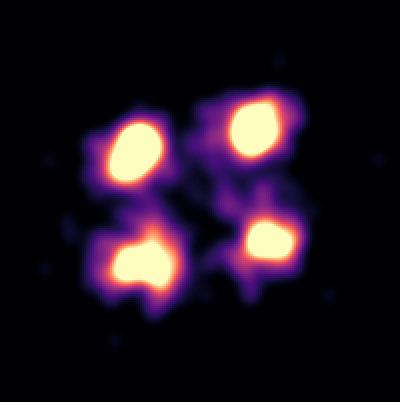
\includegraphics[width=\plotwidth]{figures/data/exp_counting/4bs_origami_1.png}
    \&
    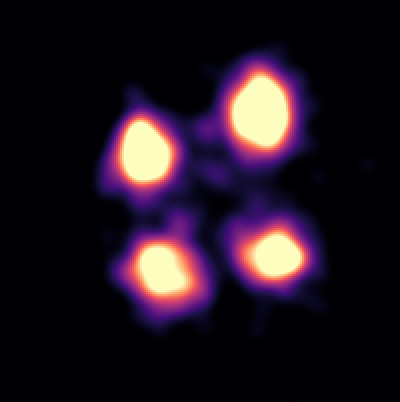
\includegraphics[width=\plotwidth]{figures/data/exp_counting/4bs_origami_2.png}
    \&
    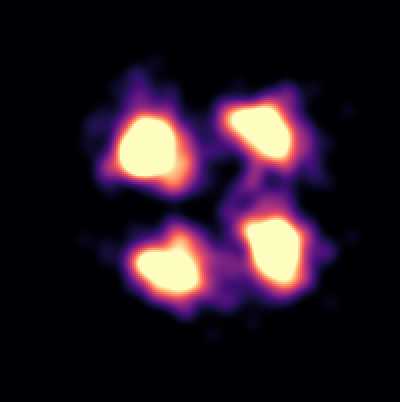
\includegraphics[width=\plotwidth]{figures/data/exp_counting/4bs_origami_3.png}
    \&
    
\includegraphics[width=\plotwidth]{figures/data/exp_counting/4bs_origami_4.png}
    \\
  };

  % scale bar
  \node[
    rectangle,
    minimum width=0.25\plotwidth, % images are 400px, 1/4 is 100px and that is 20nm
    fill=white,
    anchor=south east,
    inner sep=0pt,
    outer sep=2mm] (scalebar) at (samples-1-4.south east) {};
  \node[anchor=south,white] at (scalebar.center) {\tiny $20 \micrometer$};
\end{tikzpicture}
%
  \end{panel}
  \begin{panel}{(d)}{0.2\textwidth}
    \hspace{2mm}%
    \def\plotwidth{0.8\textwidth}%
    \def\plotheight{20mm}%
    \tikzsetnextfilename{exp_mean_probabilities_n1}%
\begin{tikzpicture}

  \pgfplotsset{every axis/.style={name=n1}}
  \def\posteriorcsv{figures/data/exp_counting/mean_probabilities.csv}
  \def\posteriorcol{n1_prob}
  \def\eps{0.001}%  skip bars for values below eps
\@ifundefined{noylabels}{}{
  \pgfplotsset{yticklabel=\empty}
  \pgfplotsset{ylabel=\empty}
}
\@ifundefined{noxlabel}{
  \pgfplotsset{xlabel=$n$}
}{
  \pgfplotsset{xlabel=\empty}
}
\begin{axis}[
  width=\plotwidth,
  height=\plotheight,
  scale only axis=true,
  enlarge x limits={abs=1.5},
  enlarge y limits=0,
  ymin=0,
  ymax=1,
  scaled ticks=false,
  ticklabel style={font=\tiny},
  xtick distance=1,
  axis background/.style={fill=white},
]

  \addplot+[
    ybar,
    bar width=1,
    mark=none,
    fill=posteriorcolor,
    fill opacity=0.6,
    draw=posteriorcolor,
    y filter/.expression={
      y < \eps ? nan : y
    },
  ] table [
    col sep=comma,
    y=\posteriorcol,
    x=n,
  ] {\posteriorcsv};

  \ifdefined\posteriorcolextra
    \addplot+[
      ybar,
      bar width=1,
      mark=none,
      fill=posteriorcolor!60!black,
      fill opacity=0.6,
      draw=posteriorcolor,
      y filter/.expression={
        y < \eps ? nan : y
      },
    ] table [
      col sep=comma,
      y=\posteriorcolextra,
      x=n,
    ] {\posteriorcsv};
  \fi

\end{axis}

  \node[anchor=south] at (n1.outer north) {origami with $\n=1$};

\end{tikzpicture}
%
  \end{panel}
  \begin{panel}{(e)}{0.2\textwidth}
    \hspace{2mm}%
    \def\plotwidth{0.8\textwidth}%
    \def\plotheight{20mm}%
    \tikzsetnextfilename{exp_mean_probabilities_n4}%
\begin{tikzpicture}

  \pgfplotsset{every axis/.style={name=n4}}
  \def\posteriorcsv{figures/data/exp_counting/mean_probabilities.csv}
  \def\posteriorcol{n4_prob}
  \def\eps{0.001}%  skip bars for values below eps
\@ifundefined{noylabels}{}{
  \pgfplotsset{yticklabel=\empty}
  \pgfplotsset{ylabel=\empty}
}
\@ifundefined{noxlabel}{
  \pgfplotsset{xlabel=$n$}
}{
  \pgfplotsset{xlabel=\empty}
}
\begin{axis}[
  width=\plotwidth,
  height=\plotheight,
  scale only axis=true,
  enlarge x limits={abs=1.5},
  enlarge y limits=0,
  ymin=0,
  ymax=1,
  scaled ticks=false,
  ticklabel style={font=\tiny},
  xtick distance=1,
  axis background/.style={fill=white},
]

  \addplot+[
    ybar,
    bar width=1,
    mark=none,
    fill=posteriorcolor,
    fill opacity=0.6,
    draw=posteriorcolor,
    y filter/.expression={
      y < \eps ? nan : y
    },
  ] table [
    col sep=comma,
    y=\posteriorcol,
    x=n,
  ] {\posteriorcsv};

  \ifdefined\posteriorcolextra
    \addplot+[
      ybar,
      bar width=1,
      mark=none,
      fill=posteriorcolor!60!black,
      fill opacity=0.6,
      draw=posteriorcolor,
      y filter/.expression={
        y < \eps ? nan : y
      },
    ] table [
      col sep=comma,
      y=\posteriorcolextra,
      x=n,
    ] {\posteriorcsv};
  \fi

\end{axis}

  \node[anchor=south] at (n4.outer north) {origami with $\n=4$};

\end{tikzpicture}
%
  \end{panel}

  \caption{
    \panelref{a, b} Experimental traces with super-resolution confirmed counts of one (a) and four (b), and \ours fits
    %
    \panelref{c} Super-resolution visualization of origamis made with four binding sites.
    %
    \panelref{d, e} Average \ours posterior distributions of 112 traces with a known $n$ of one (d) and 
    110 traces with a known $n$ of four (e)
  }
  \label{fig:results:experimental}
\end{figure*}


\end{document}
